\documentclass[11pt,notes=hide,aspectratio=169,mathserif]{beamer}

% PACKAGES
\usepackage{graphics}  % Support for images/figures
\usepackage{graphicx}  % Includes the \resizebox command
\usepackage{url}	   % Includes \urldef and \url commands
\usepackage{natbib}
\usepackage{bibentry}  % Includes the \nobibliography command
\usepackage{verbatim}  %Supports comments
\usepackage{booktabs} %Supports \toprule, \bottomrule, etc in tables
\usepackage{etoolbox}  %Supports toggle commands
\usepackage{datetime}
\usepackage{bm}	%Supports bold math \bm
\usepackage{subcaption} %Supports subfigures
% PACKAGES (that should already be included by your LyX document settings)
\usepackage{amsfonts}  % Lots of stuff, including \mathbb 
\usepackage{amsmath}   % Standard math package
\usepackage{amsthm}    % Includes the comment functions

% CUSTOM DEFINITIONS
\def\newblock{} %Get beamer to cooperate with BibTeX
\linespread{1.2}

% IDENTIFYING INFORMATION
\title[class]{ECON 326: Economics of Developing Countries \\ TA Session 1}
\author[vaidehi's class ]{Vaidehi Parameswaran (Northwestern Econ)}
\date{\monthname[\the\month] \the\year}

% THEMATIC OPTIONS
%\setbeamercovered{transparent}
\usetheme{metropolis}
\definecolor{mycolor}{RGB}{48,7,144} 
\setbeamercolor{frametitle}{bg=mycolor, fg=white} % Frame title color
\setbeamercolor{title separator}{fg=mycolor} 
\setbeamercolor{progress bar}{fg=mycolor} 
\beamertemplatenavigationsymbolsempty
\setbeamertemplate{footline}[frame number]{}
\setbeamertemplate{itemize item}{\small\raisebox{1pt}{\textcolor{mycolor}{$\blacktriangleright$}}}
\setbeamertemplate{itemize subitem}{\footnotesize\raisebox{1pt}{\textcolor{mycolor}{$\triangleright$}}}
\setbeamertemplate{itemize subsubitem}{\tiny\raisebox{1pt}{\textcolor{mycolor}{$\triangleright$}}}

% BACKUP SLIDE NUMBERING
\usepackage{appendixnumberbeamer}

\begin{document}

%---------------------------------------------------------------------
\begin{frame}[plain]
\titlepage
\end{frame}
%---------------------------------------------------------------------

\section{Today}
%---------------------------------------------------------------------
\begin{frame}
    
\frametitle{Today}
\begin{itemize}
\vspace{-.3cm}
\item Introductions 
\medskip
\item Stata: \smallskip
\begin{enumerate}
    \item The basics
    \smallskip
    \item Data management
    \item Data visualisation
    \item Data analysis (OLS, Binary variables)
\end{enumerate}
\end{itemize}
\end{frame}
%---------------------------------------------------------------------

\section{Introductions}
%---------------------------------------------------------------------
\begin{frame}{Introductions}
\begin{itemize}
\item Me: a second-year grad student in the econ department 
\begin{itemize}
        \item I hope to study labour markets, monopsony power in India 
        \item Email: \textcolor{blue}{vaidehiparameswaran2029@u.northwestern.edu} 
        \item Office hours: Monday 2-3pm in KGH 3411, Friday 2-3pm over zoom
\end{itemize}
\end{itemize}
\end{frame}
%---------------------------------------------------------------------

\section{Stata Basics}
%---------------------------------------------------------------------
\begin{frame}{Why Stata?}
Advantages of Stata: 
    \begin{itemize}
        \item \textbf{Easy to use}: you won't need to spend much time updating it, installing packages, or debugging your code (relative to, e.g., R and Python) 
        \item \textbf{Well documented}: you can figure out how any command works writing \texttt{help} (or just \texttt{h}) into the prompt, followed by the command's name
        \item \textbf{Widely used}: Stata has a lot of built-in commands for the kind of econometrics you'll be doing in this class and is widely used in applied micro research
    \end{itemize}
\end{frame}
%---------------------------------------------------------------------

%---------------------------------------------------------------------
\begin{frame}{Disadvantages of Stata}
\begin{itemize}
    \item \textbf{Cost}: Stata is not free, but you can access it through the university
    \item \textbf{Not open source}: Needs a license, can't see the source code 
    \item \textbf{Limited for tasks like ML}: If you're interested in machine learning, you might want to learn R or Python
\end{itemize}
\end{frame}
%---------------------------------------------------------------------

%---------------------------------------------------------------------
\begin{frame}{The Interface}
    \begin{itemize}
    \item Open Stata to see the \textbf{Results Window}
        \begin{figure}
            \centering
            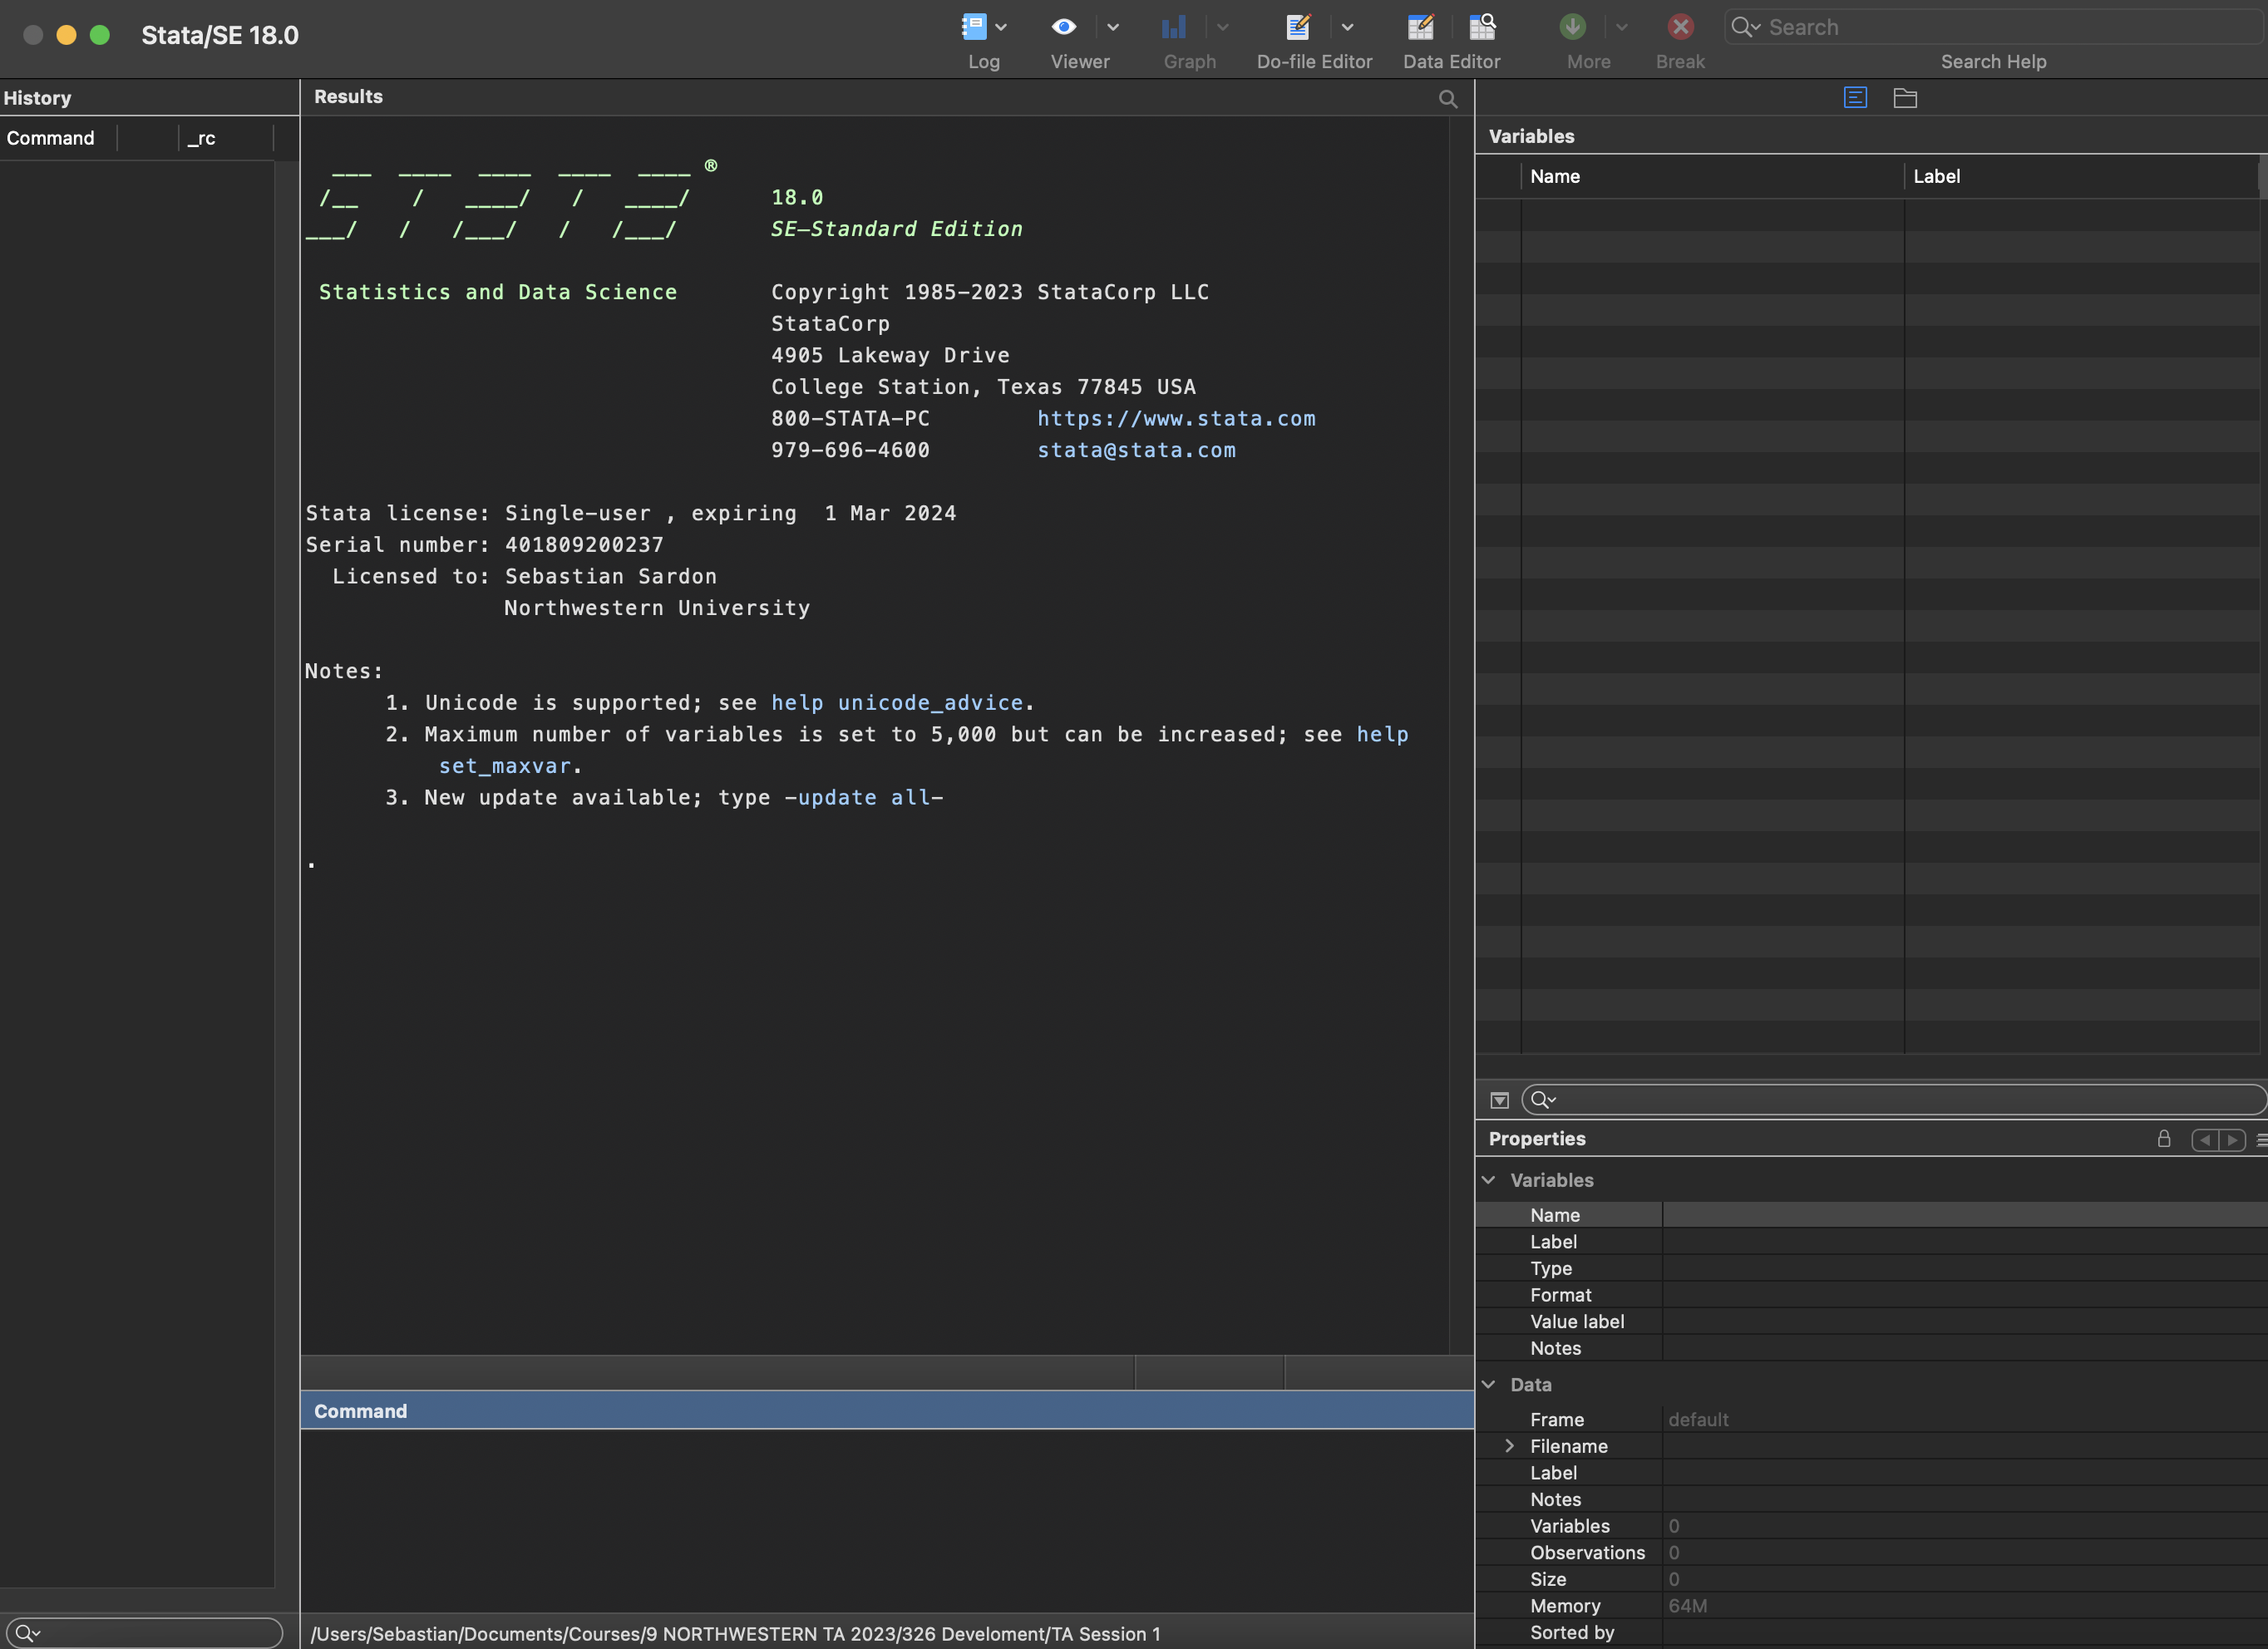
\includegraphics[width=0.5\textwidth]{inputs/ta1_result_window1.png}
        \end{figure}
    \end{itemize}
\end{frame}
%---------------------------------------------------------------------

%---------------------------------------------------------------------
\begin{frame}{The Interface}
\begin{itemize}
\item \textbf{Command Prompt:} allows you to type and run commands (try ``\texttt{di}'' followed by what you want Stata to display)
\end{itemize}
\begin{figure}
    \centering
    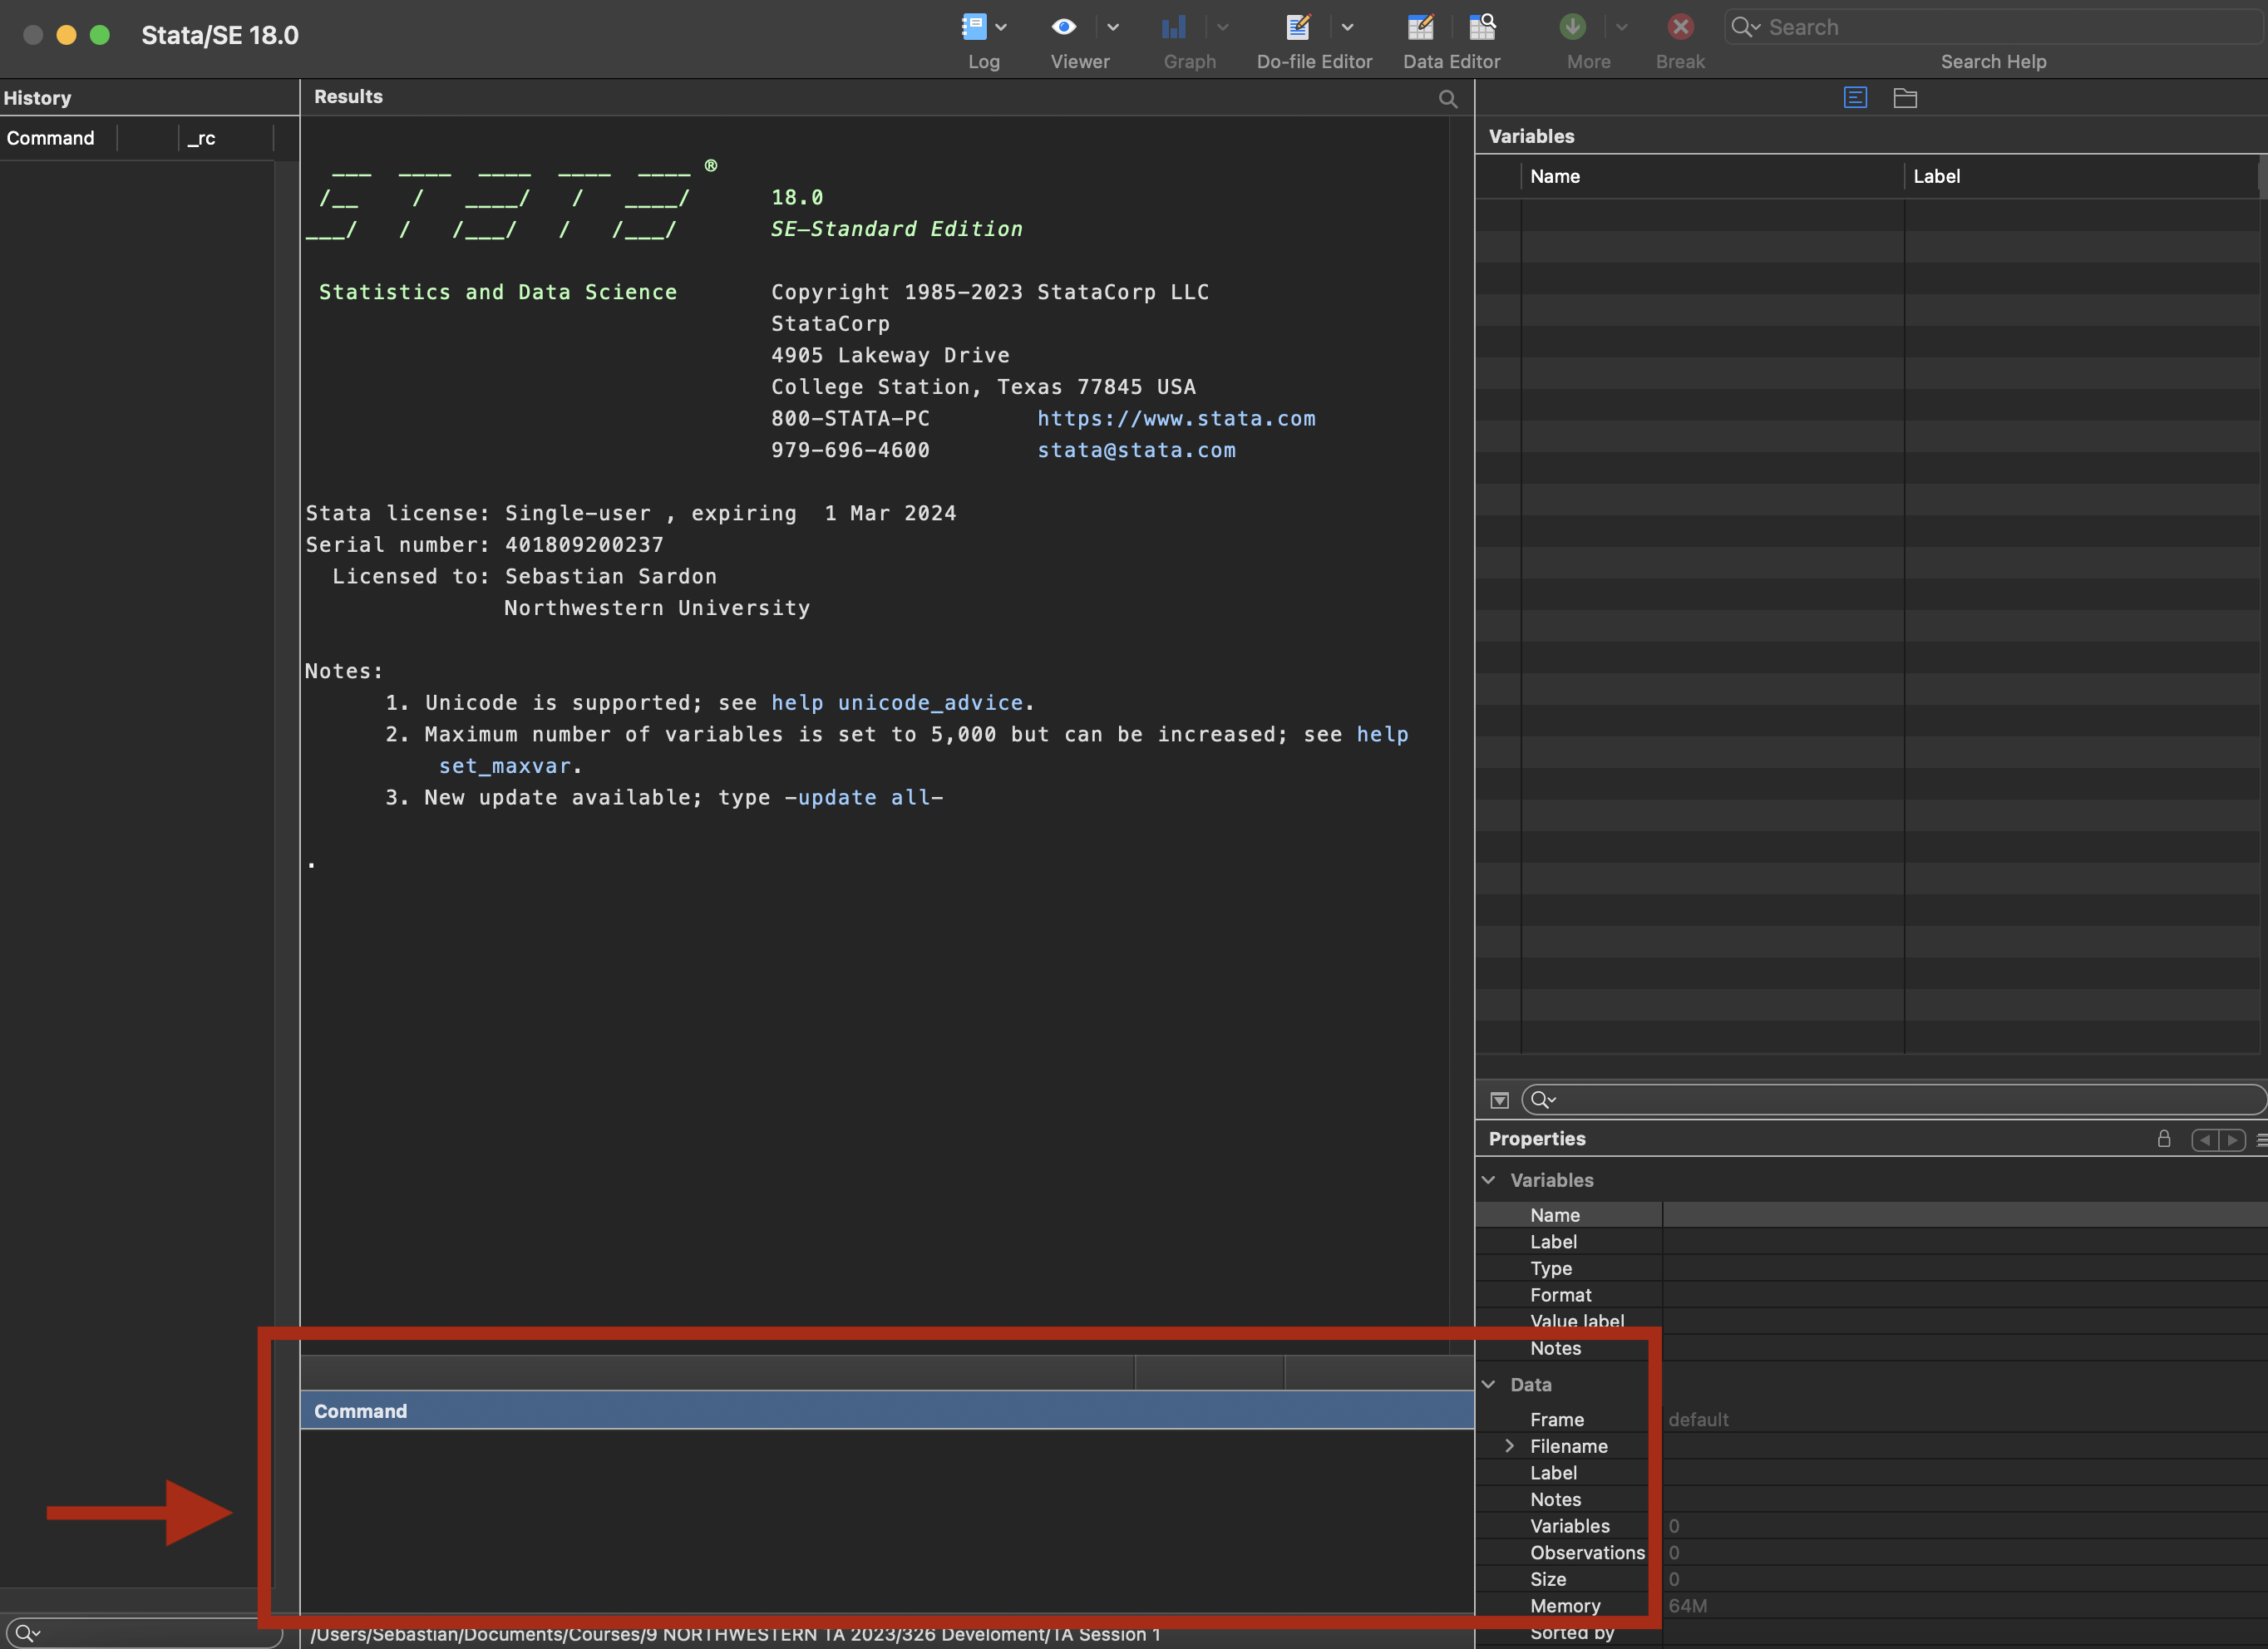
\includegraphics[width=0.5\textwidth]{inputs/ta1_result_window2.png}
\end{figure}
\end{frame}
%---------------------------------------------------------------------

%---------------------------------------------------------------------
\begin{frame}{The Interface}
\begin{itemize}
\item \textbf{Results} panel will contain the output of all executed commands
\end{itemize}
\begin{figure}
    \centering
    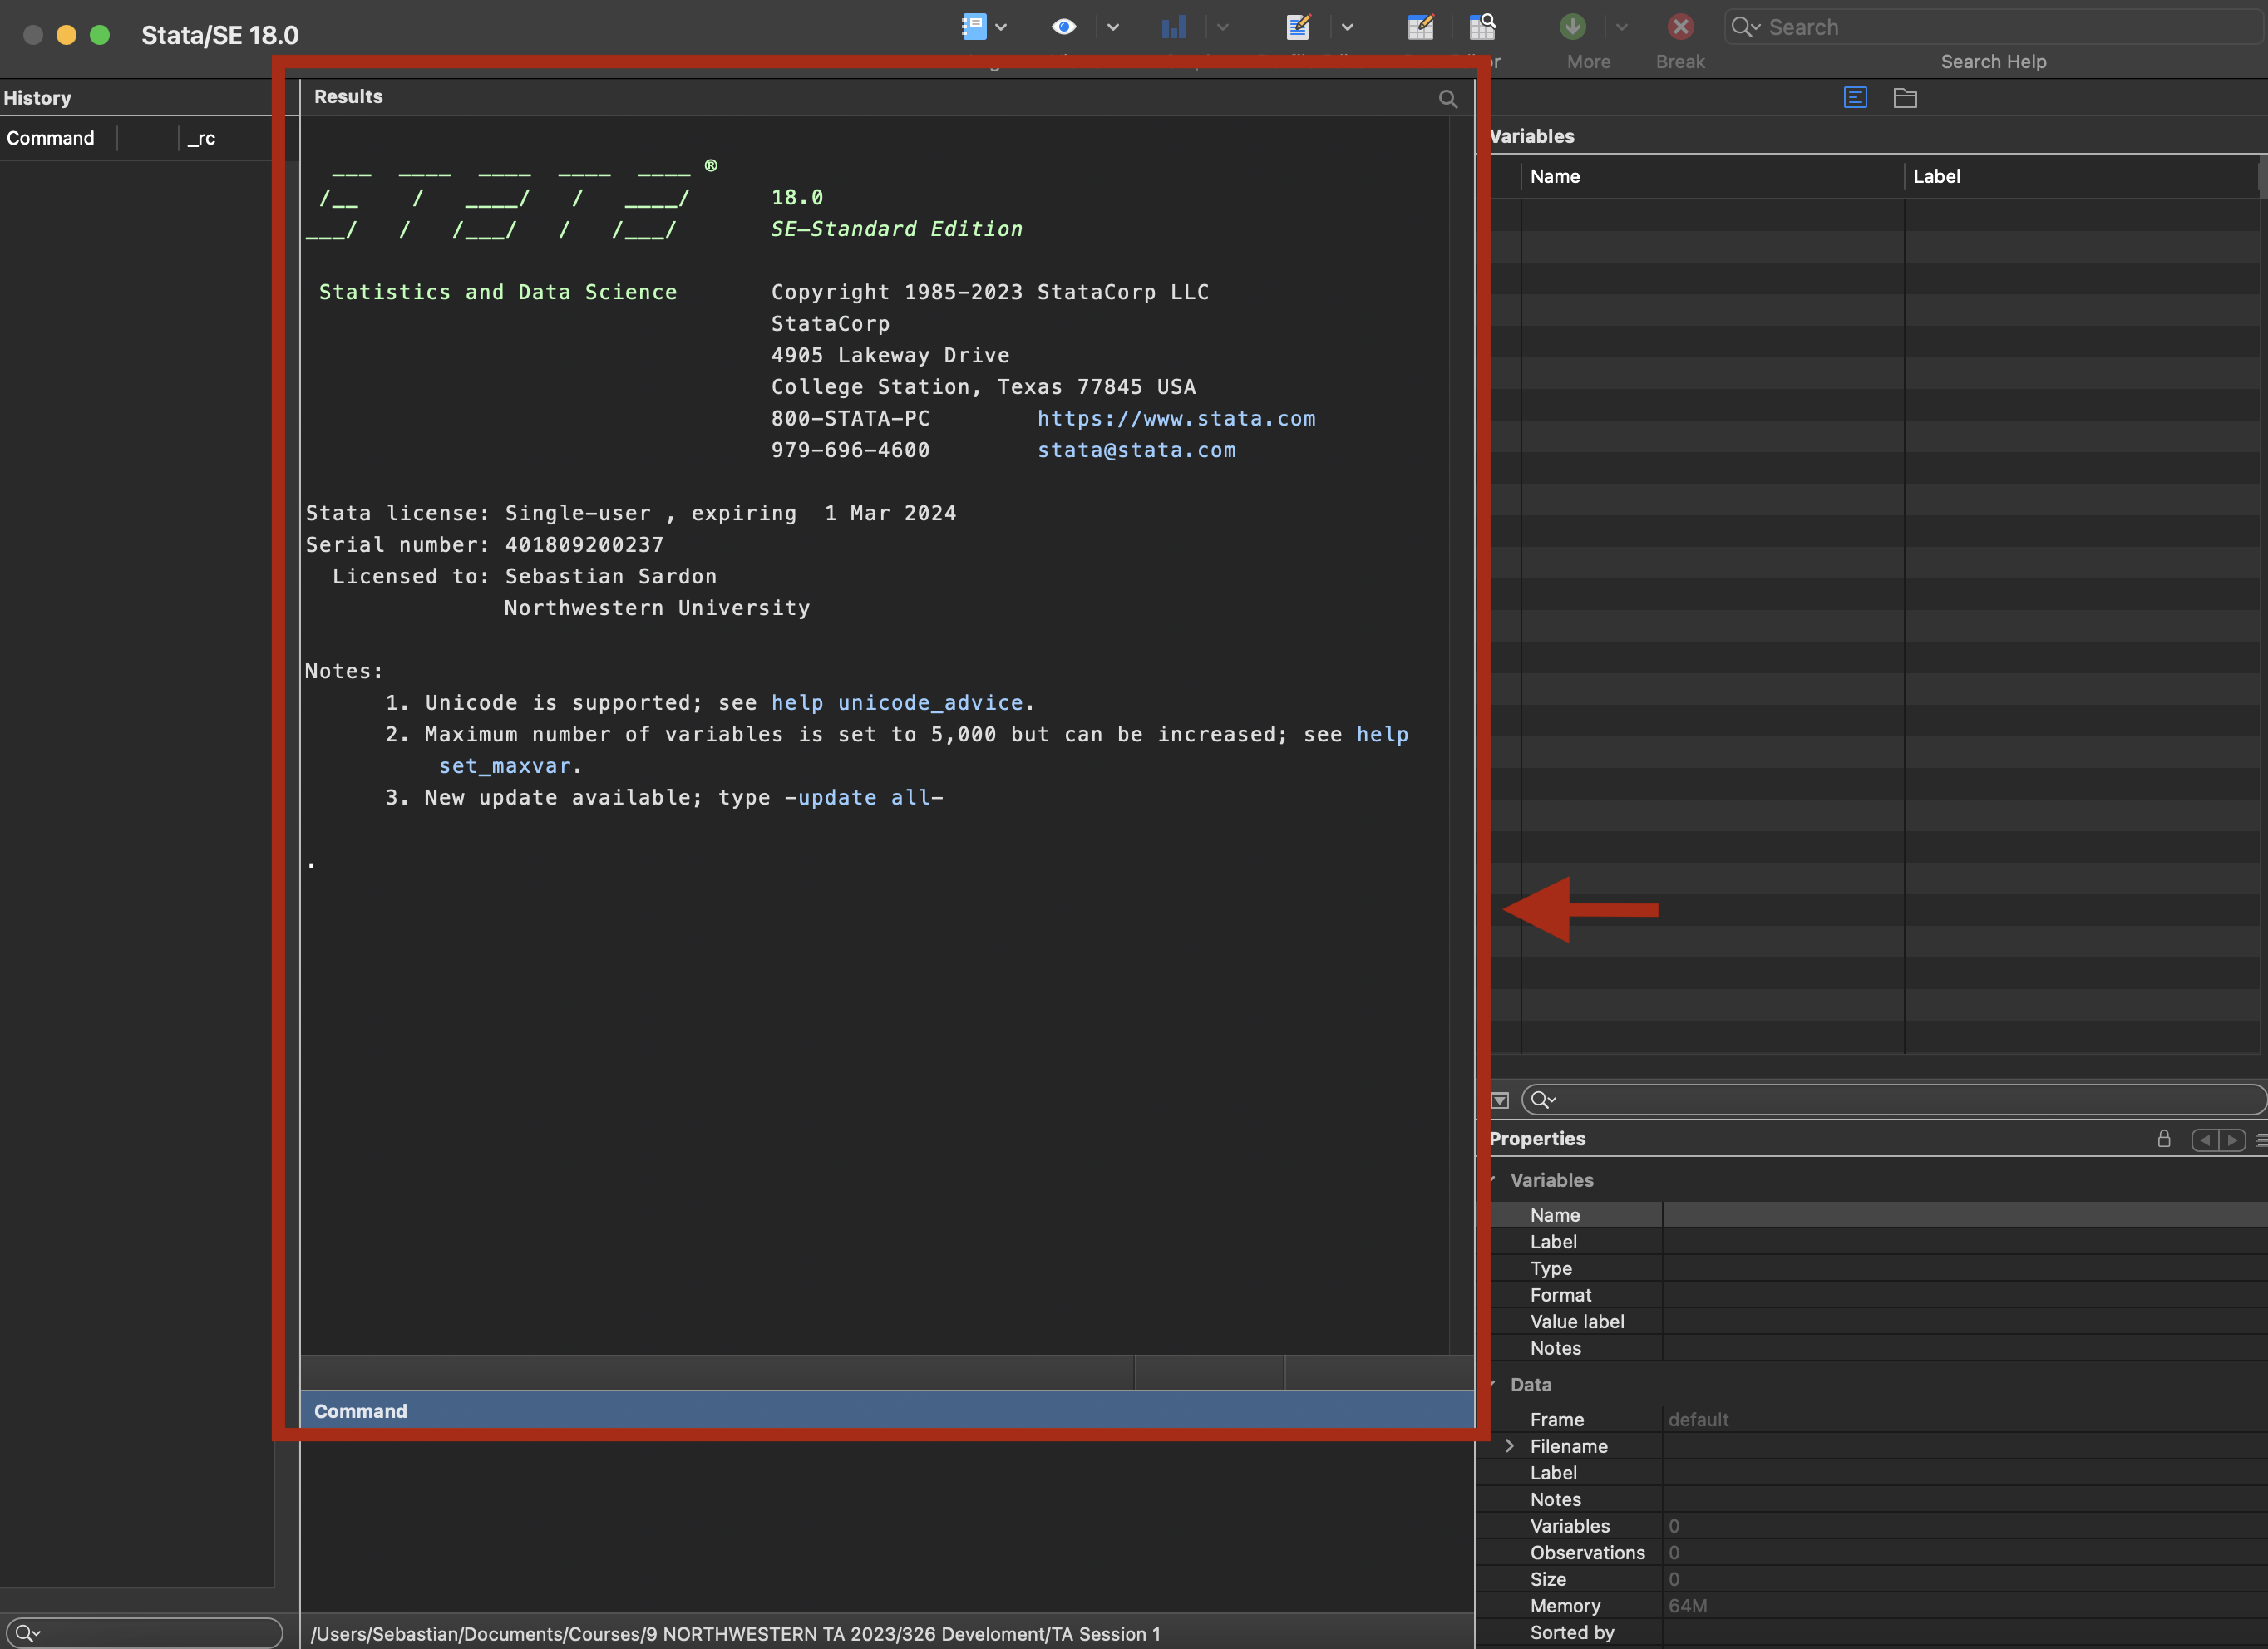
\includegraphics[width=0.5\textwidth]{inputs/ta1_result_window3.png}
\end{figure}
\end{frame}
%---------------------------------------------------------------------

%---------------------------------------------------------------------
\begin{frame}{The Interface}
    \begin{itemize}
        \item \textbf{History} panel will list all commands sent to the prompt
        \end{itemize}
    \begin{figure}
        \centering
        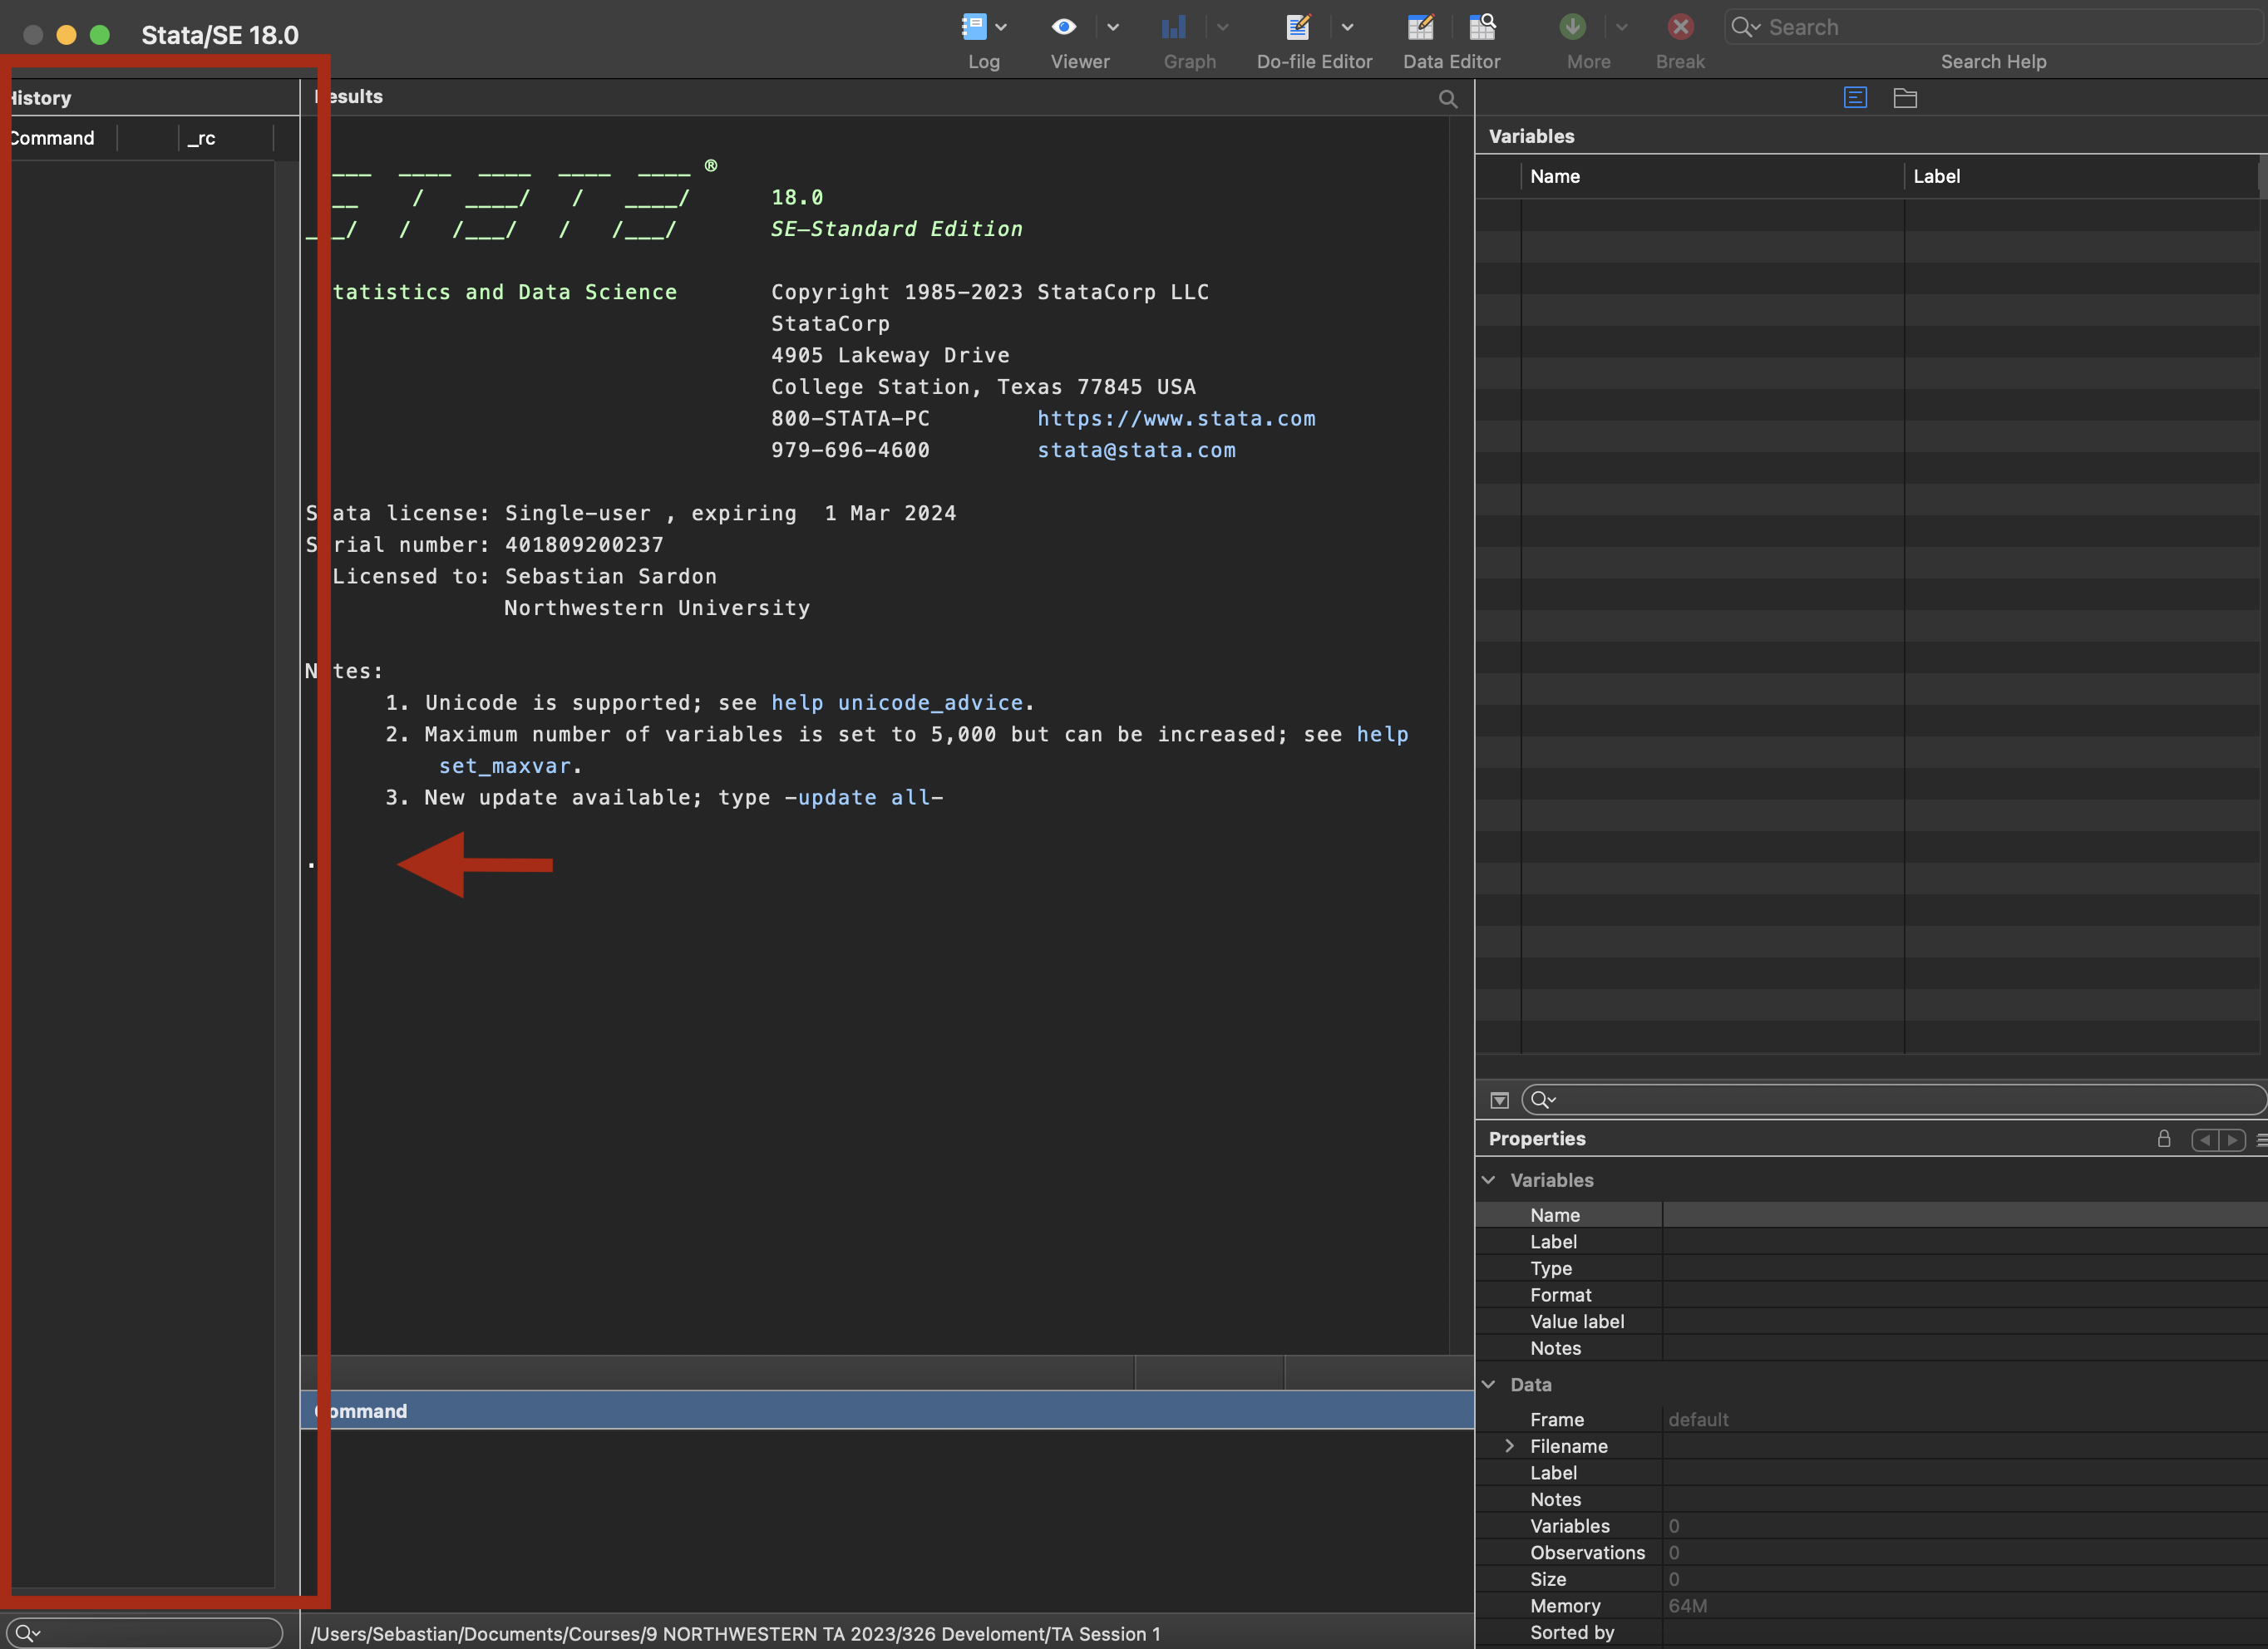
\includegraphics[width=0.5\textwidth]{inputs/ta1_result_window4.png}
    \end{figure}
\end{frame}
%---------------------------------------------------------------------

%---------------------------------------------------------------------
\begin{frame}{The Interface}
    \begin{itemize}
        \item \textbf{Variables} panel will show you all variables in the dataset that's currently open
    \end{itemize}
    \begin{figure}
        \centering
        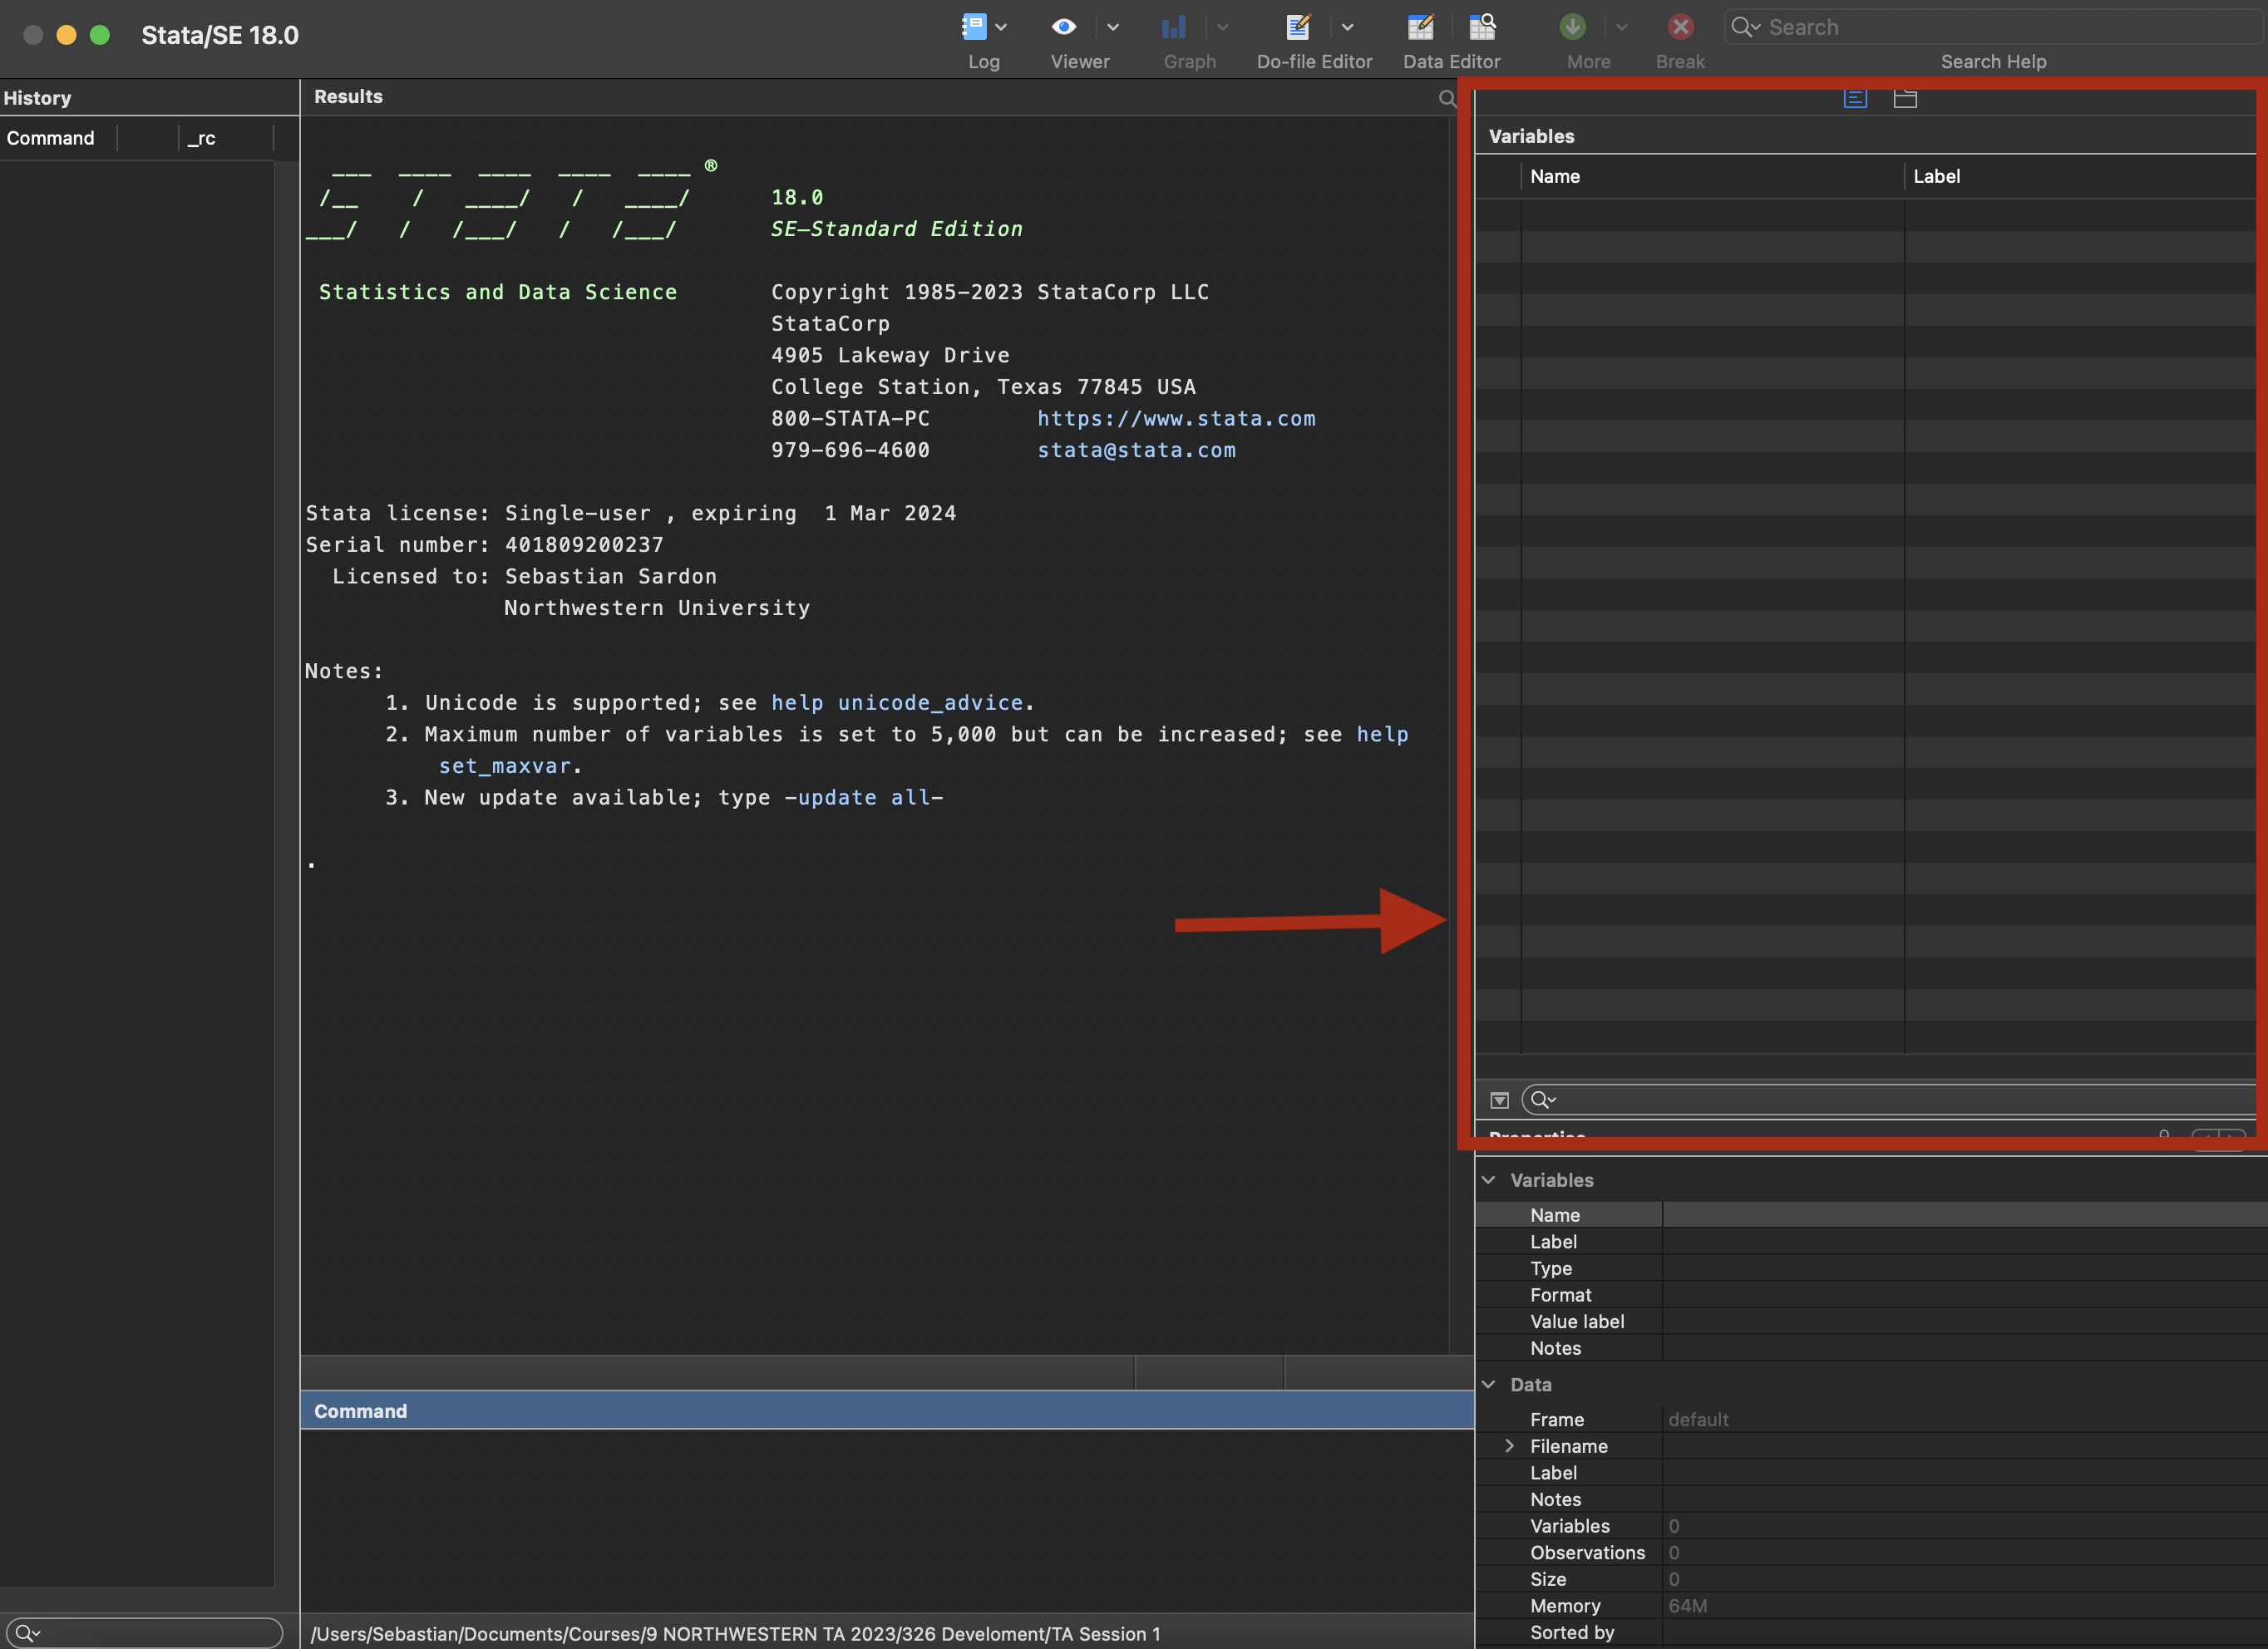
\includegraphics[width=0.5\textwidth]{inputs/ta1_result_window5.png}
    \end{figure}
\end{frame}
%---------------------------------------------------------------------

%---------------------------------------------------------------------
\begin{frame}{The Interface}
\begin{itemize}
    \item \textbf{Properties} panel will show additional information about the currently open dataset
\end{itemize}
\begin{figure}
    \centering
    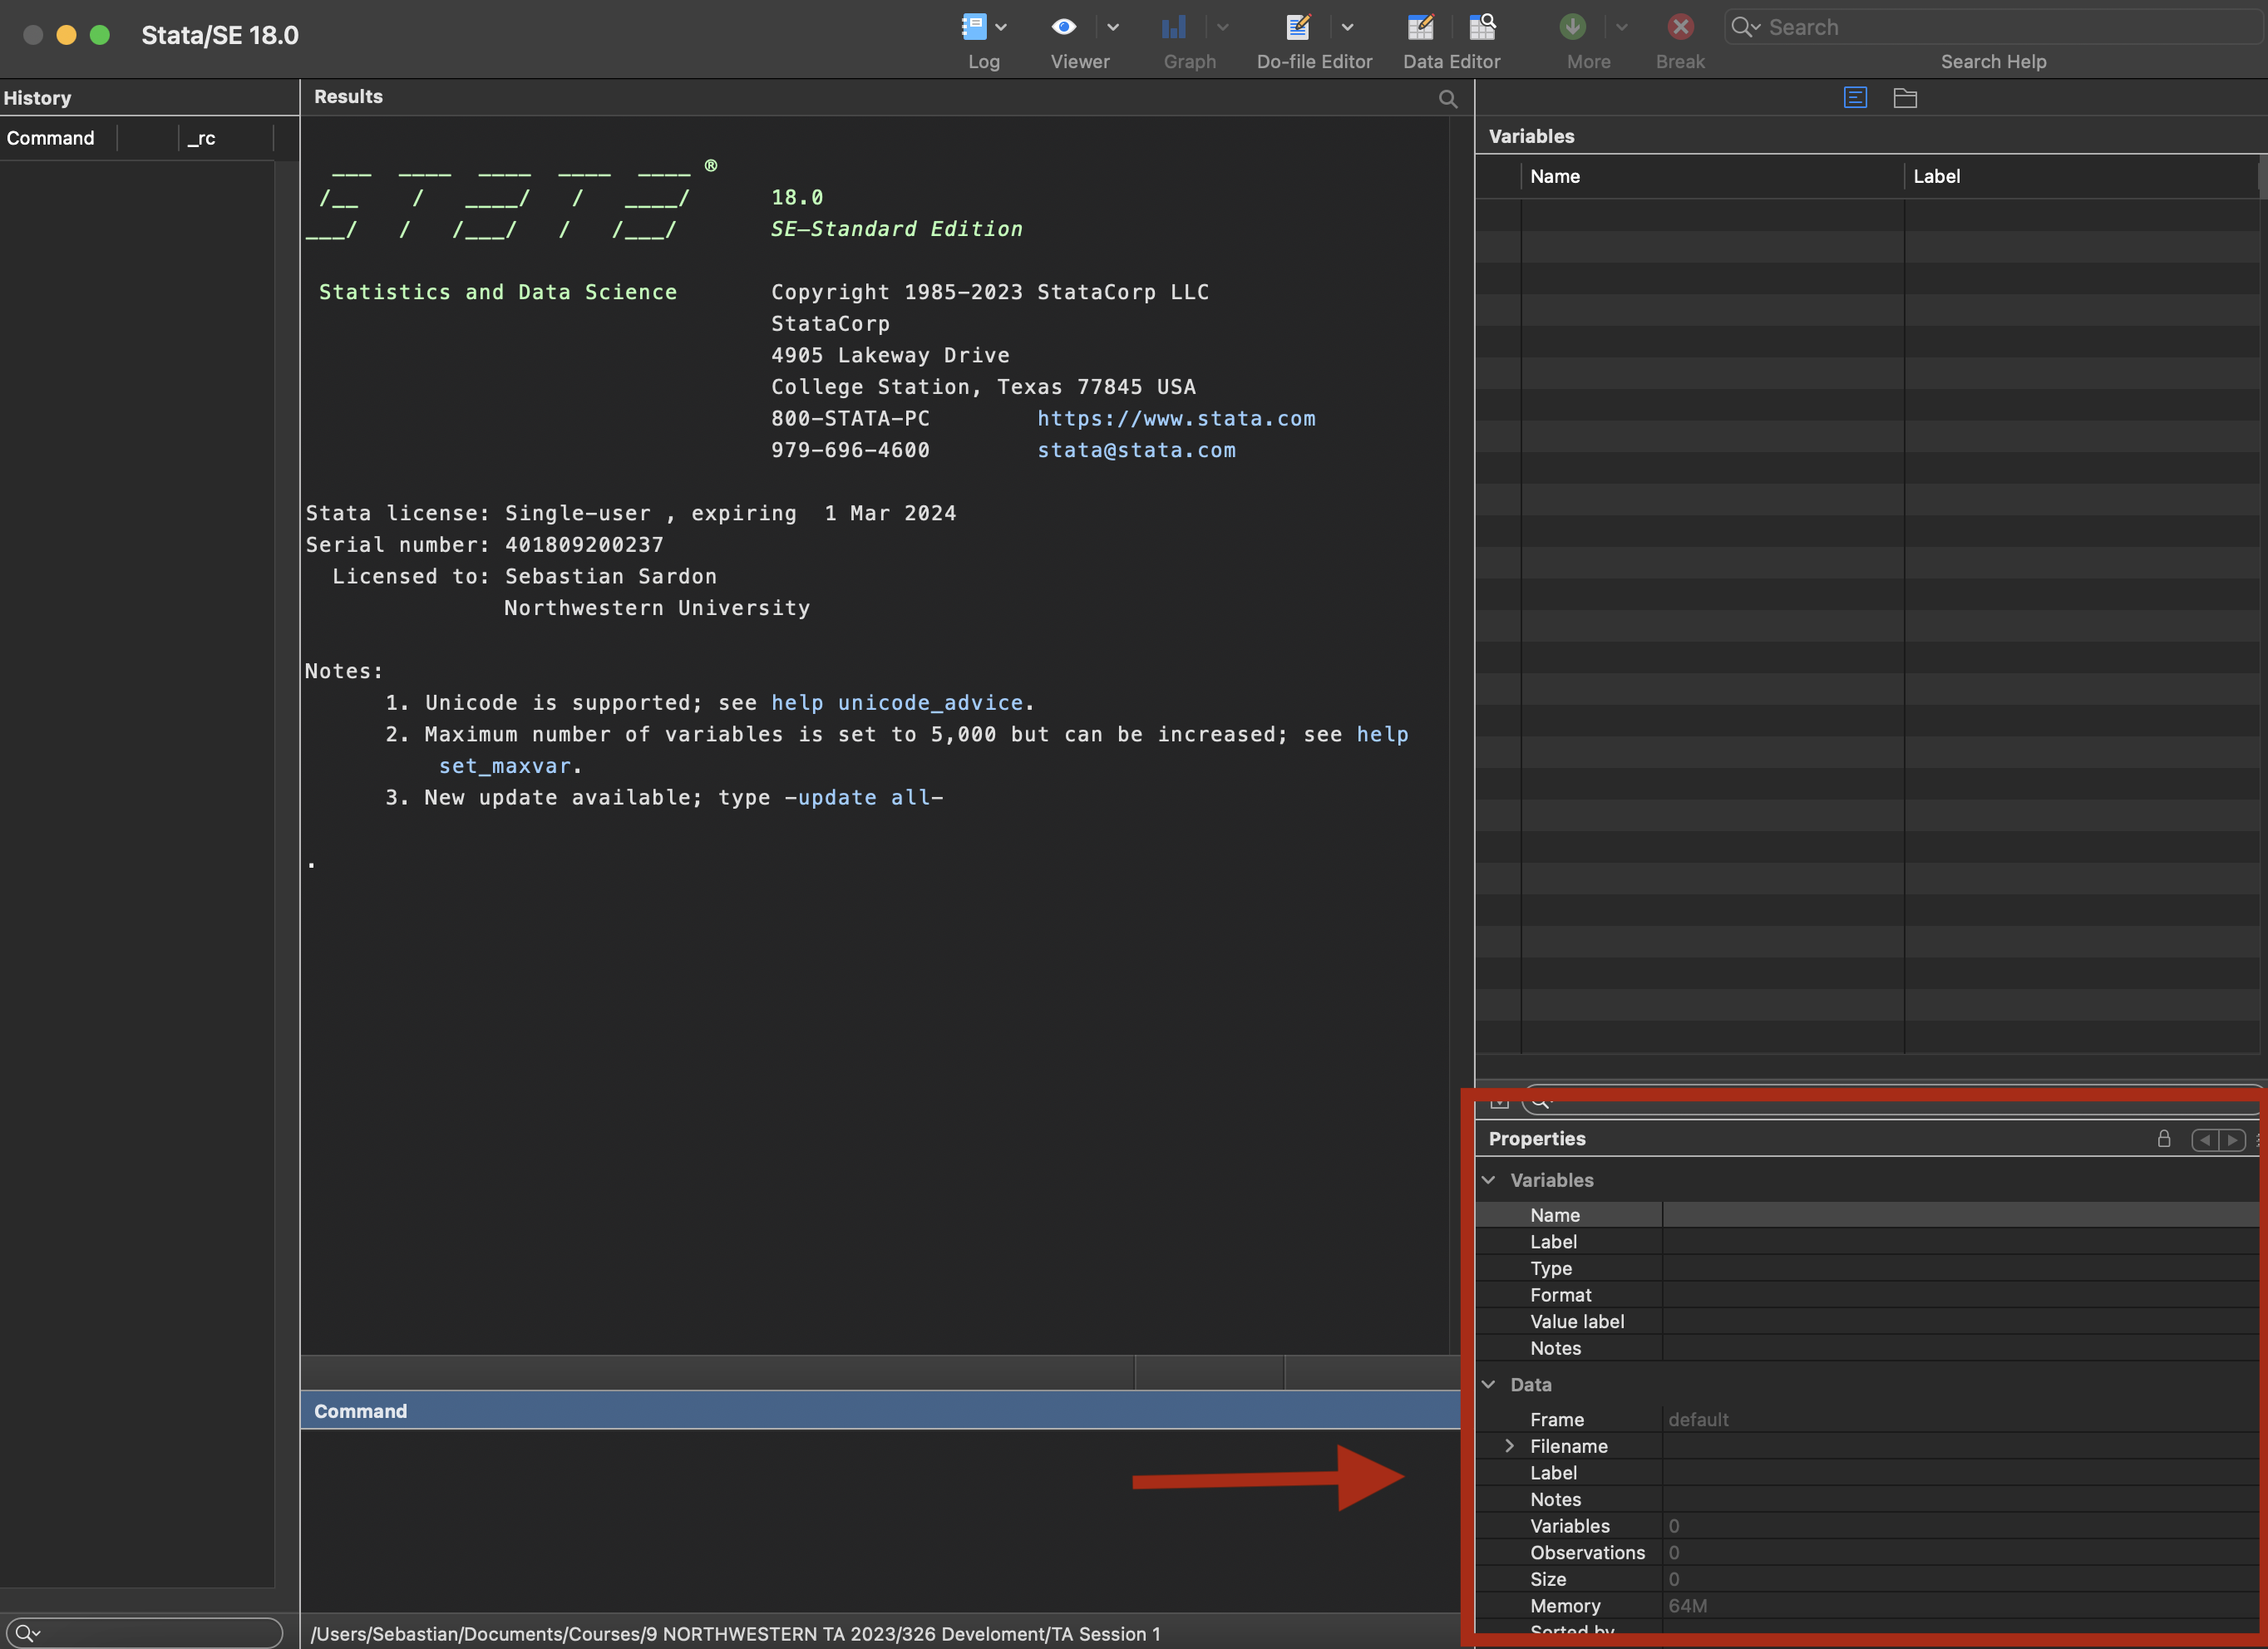
\includegraphics[width=0.5\textwidth]{inputs/ta1_result_window6.png}
\end{figure}
\end{frame}
%---------------------------------------------------------------------

%---------------------------------------------------------------------
\begin{frame}{The Interface}
    \begin{itemize}
    \item There's also a \textbf{Data Editor} window that allows you to visualize the currently open dataset 
    \item To open it, use the \texttt{br} command
        \begin{figure}
            \centering
            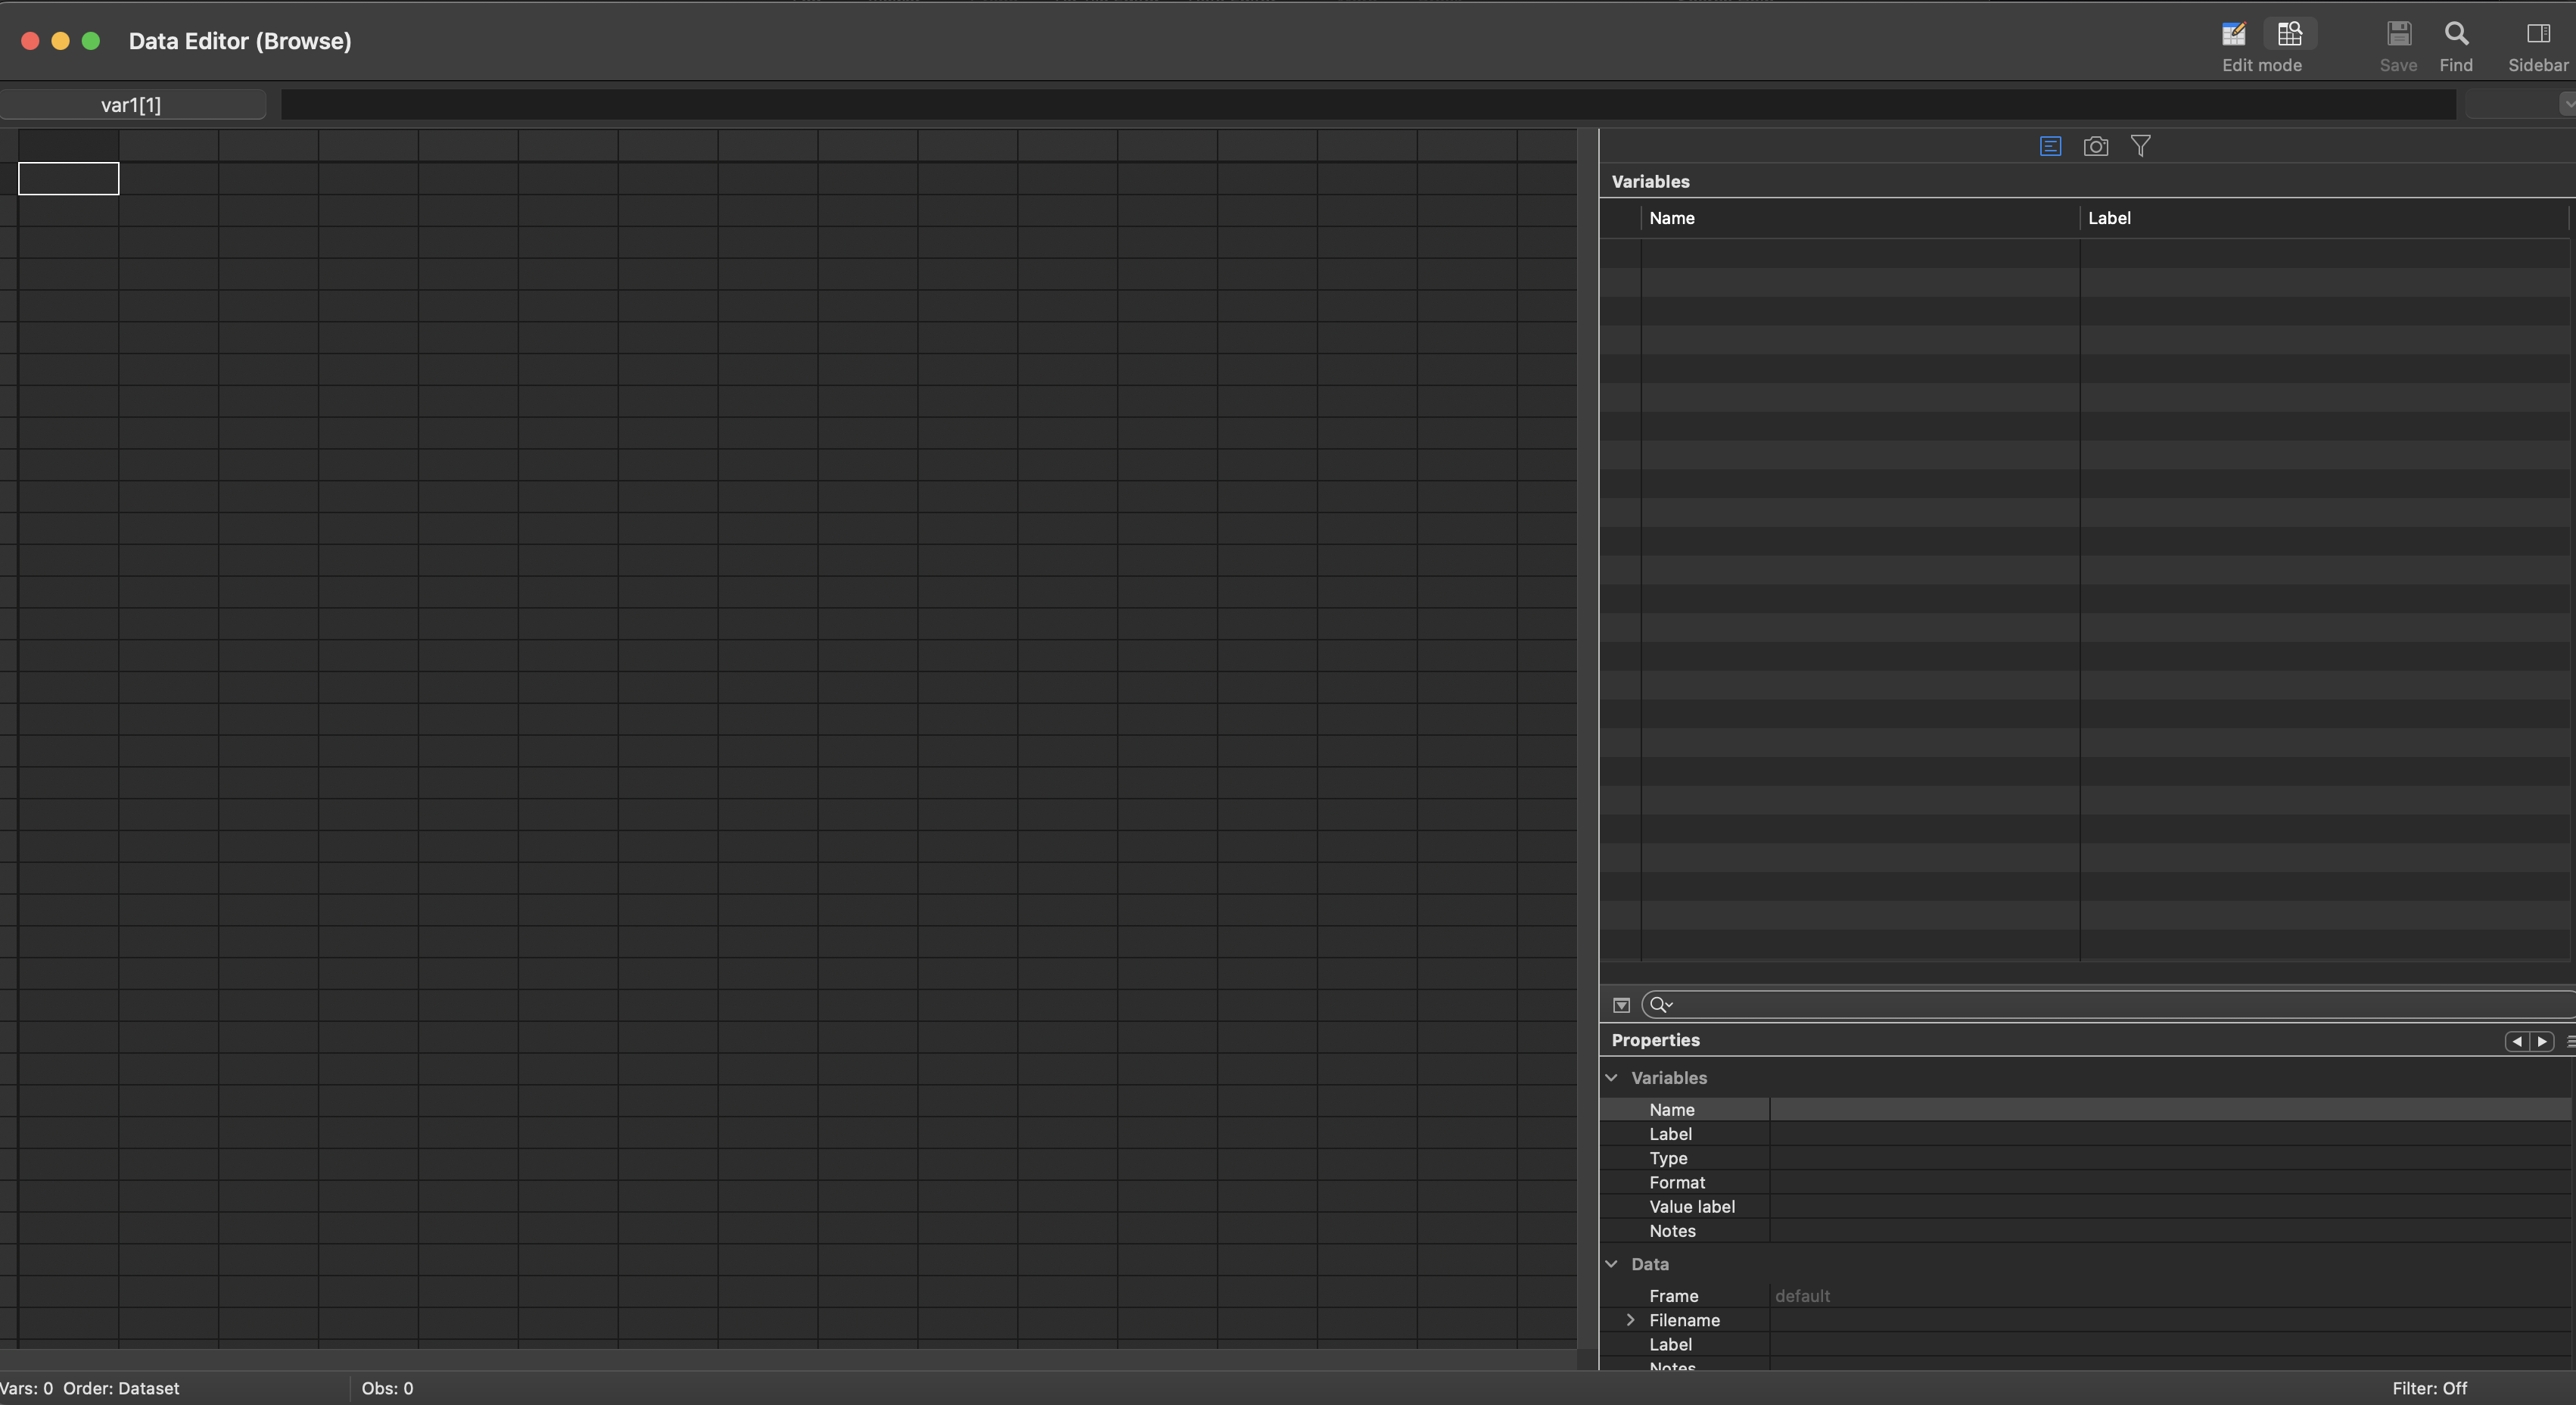
\includegraphics[width=0.6\textwidth]{inputs/ta1_stata_data.png}
        \end{figure}
    \end{itemize}
\end{frame}
%---------------------------------------------------------------------

%---------------------------------------------------------------------
\begin{frame}{The Interface}
    \begin{itemize}
    \item The \textbf{Do-File Editor} is where we do most of our work
    \item A highly optimized text editor for writing Stata code
    \item You open it by opening any \texttt{.do} file, or in the menu bar via \textbf{File$\rightarrow$ New $\rightarrow$ Do-file}.
    \item You can select the lines you want to run, then run them with \textbf{Shift$+$CMD$+$D} (Mac) or \textbf{CTRL$+$D} (Windows)
    \item Use the same shortcut keys without selection to run the entire do-file
    \end{itemize}
\end{frame}
%---------------------------------------------------------------------

%---------------------------------------------------------------------
\begin{frame}{Writing code in Stata}
    \begin{itemize}
        \item Usual Preamble: typically start any do-file with these 4 commands\smallskip
        \begin{enumerate}
            \item  \texttt{clear all} $\rightarrow$ \textcolor{blue}{Drops all variables}\smallskip
            \item  \texttt{cd "/Users/vaidehiparameswaran/Desktop/teaching/econ326-sp/"} $\rightarrow$ \textcolor{blue}{Change Directory: this indicates where you will open from and save your files. All paths in the dofile will automatically get this prefix.}\smallskip
            \item \texttt{capture log close } $\rightarrow$ \textcolor{blue}{*If* a log file was opened, this closes it. \textcolor{black}{\texttt{capture}} suppresses output and potential error messages which would terminate the dofile. Here, we'd get an error the first time we run the dofile: no log would be open.}\smallskip
            \item \texttt{log using TA1.txt, replace } $\rightarrow$ \textcolor{blue}{Opens a log file (called \textcolor{black}{\texttt{TA1}}) that will record the contents of the Results window. This lets others verify your code actually worked. }\smallskip
        \end{enumerate}
    \end{itemize}
\end{frame}
%---------------------------------------------------------------------

%---------------------------------------------------------------------
\begin{frame}{Comment your code}
    \begin{itemize}
        \item This means writing notes that won't run as commands, useful to annotate do-file and divide into sections \medskip
        \item Two ways to comment your code:\smallskip
        \begin{itemize}
            \item Typing \textcolor{red}{\texttt{*}} at the beginning of a line allows you to comment \smallskip
            \item You can also insert a comment after a command line by adding \textcolor{red}{\texttt{//}} after the command\smallskip
            \item Example: \smallskip
                    \end{itemize}
            $$\footnotesize \texttt{display("Hello World!") \textcolor{red}{//This line prints statement in results window}}$$
    \end{itemize}
\end{frame}
%---------------------------------------------------------------------

%---------------------------------------------------------------------
\begin{frame}{Stata does math}
\begin{itemize}
    \item Operators: \texttt{display} (or equivalently, \texttt{di}) also works as a calculator \smallskip
    \begin{itemize}
        \item \texttt{display $2*3 + 3/2 - 2^{\wedge} 3$} $\rightarrow$ \textcolor{blue}{This will give you -0.5. Notice Stata follows the standard order of operations so you don't need brackets unless you want to change their order.}
    \end{itemize}\bigskip
    \item Mathematical functions\smallskip
\begin{itemize}
\item \texttt{display ln(sqrt(abs(-2)))} $\rightarrow$ \textcolor{blue}{This will give you 0.34657359, the result of $\log(\sqrt{|-2|})$. } 
\end{itemize}
\end{itemize}
\end{frame}
%---------------------------------------------------------------------

%---------------------------------------------------------------------
\begin{frame}{String Functions}
\begin{itemize}
\item \textbf{string variables} are those containing letters (and other characters) instead of numbers (e.g. country names). You use string functions to manipulate them: \medskip
        \begin{itemize}
        \item \texttt{display substr("abc",1,2)} $\rightarrow$ \textcolor{blue}{This tells Stata that, starting from position 1, in the string ``abc'', i.e. starting from ``a'', it should keep 2 characters. The result would be ``ab''.} \smallskip
        \item \texttt{display subinstr("abc","b","X",1)} $\rightarrow$ \textcolor{blue}{This tells Stata to replace a substring (``b'') within a string (``abc'') with another substring(``X''). The last argument, ``1'', indicates how many times such replacements are going to be made. Here ``b'' only occurs once within the string so this does not matter. The result would be ``aXc''. }\smallskip
        \item \textcolor{blue}{If we replace the ``1'' from above with a period, we are telling Stata to do the replacement as many times as possible. For example:} \texttt{display subinstr("abcbb","b","X",.)} \textcolor{blue}{yields ``aXcXX''}. 
    \end{itemize}
\end{itemize}    
\end{frame}
%---------------------------------------------------------------------

%---------------------------------------------------------------------
\begin{frame}{Data Management}
\begin{itemize}
    \item We will work with NLS data on wage and education 
    \item To begin, run the preamble commands
    \item Then open the data:
    $$\texttt{use "rawdata.dta", clear }$$ 
    \item The \texttt{use} command opens the data set from the directory you set earlier in the preamble with \texttt{cd}
    \item \texttt{clear} is an option that specifies that it is okay to replace the dataset in memory. You need to include this to avoid errors in case you already had a dataset loaded into Stata
    \item \textbf{In general, a comma will separate a Stata command and its options}
\end{itemize}
\end{frame}
%---------------------------------------------------------------------

%---------------------------------------------------------------------
\begin{frame}{Understanding your data}
\begin{itemize}
    \item \texttt{describe} $\rightarrow$ \textcolor{blue}{Overview of all your variables (types, formats and labels)}
    \item \texttt{codebook} $\rightarrow$ \textcolor{blue}{Prints the codebook of your data with a description of each variable}
    \item \texttt{browse} or \texttt{br} $\rightarrow$ \textcolor{blue}{Navigate dataset as if it was an Excel spreadsheet}
    \item \texttt{count}   $\rightarrow$ \textcolor{blue}{Total number of observations in your data}
\end{itemize}
\end{frame}
%---------------------------------------------------------------------

%---------------------------------------------------------------------
\begin{frame}{Understanding the data}
\begin{itemize}
\item \texttt{tabulate x}   $\rightarrow$ \textcolor{blue}{This command gives you a frequency table for the variable specified}
\item \texttt{tabulate x y} $\rightarrow$ \textcolor{blue}{A 2 by 2 frequency table. The first variable will be displayed in the rows and the second in columns} 
\item \texttt{sum x}   $\rightarrow$ \textcolor{blue}{summarize  statistics of the variable \textcolor{black}{\texttt{x}} (short version: number of observations, mean, standard deviation, min, max)} 
\item \texttt{sum x, d}   $\rightarrow$ \textcolor{blue}{detailed version of \textcolor{black}{\texttt{sum}}, useful to inspect the distribution of a variable}
\end{itemize}
\end{frame}
%---------------------------------------------------------------------

% %---------------------------------------------------------------------
% \begin{frame}{Part 2: Data Management -- Merging Two Datasets}
%     \begin{itemize}
%     \item \texttt{merge 1:1 shortnam using "PWT\_1995.dta"} $\rightarrow$ \textcolor{blue}{Merge the current data with a new one, \textcolor{black}{\texttt{PWT\_1995.dta}} (Penn World Tables data for 1995).}
%     \begin{itemize}
%         \item Stata matches rows in both datasets with the \textbf{exact} same value of \texttt{shortnam} (country code). \item The merge is specified as \texttt{1:1}, meaning that Stata will connect each row in the current dataset (called ``master'' dataset) to \textbf{at most} one row in ``PWT.dta'' (the ``using'' dataset). 
%         \item A \texttt{1:1} merge will only work if  \texttt{shortnam} uniquely identifies rows in both datasets. So, if many rows share a country code, the merge fails.
%         \item If successful, Stata displays how many rows in the master and the using dataset were succesfully matched. Unmatched rows will also be present in the merged dataset, but they'll only have data for variables from their dataset of origin.
%         \item  Stata creates a variable called \texttt{\_merge} that encodes this information. It takes the following values:
%         \begin{itemize}
%             \item 1 for unmatched rows in the master dataset
%             \item 2 for unmatched rows in the using dataset
%             \item 3 for matched rows.
%         \end{itemize}
%         \item Stata also allows many to one (\texttt{m:1}) and one to many (\texttt{1:m}) merges.
%     \end{itemize}
% \end{itemize}
% \end{frame}
% %---------------------------------------------------------------------

%---------------------------------------------------------------------
\begin{frame}{Generating Variables}
\begin{itemize}
     \item \texttt{gen lwage = ln (wage)}  $\rightarrow$ \textcolor{blue}{The \texttt{gen} command generates new variables} 
     \item \texttt{drop lwage}  $\rightarrow$ \textcolor{blue}{The \texttt{drop} command deletes variables} 
     \item \texttt{gen lwage = ln(wage) if educ >= 13}  
     \item \texttt{replace lwage = ln(wage) if educ < 13} 
     \item \texttt{label var lwage "log wages"}  $\rightarrow$ \textcolor{blue}{The \texttt{label var} command labels variables} 
\end{itemize}
\end{frame}
%---------------------------------------------------------------------

%---------------------------------------------------------------------
\begin{frame}{Saving your work!}
    \begin{itemize}
        \item \texttt{cap mkdir output}	$\rightarrow$ \textcolor{blue}{create a folder (directory) called \textcolor{black}{\texttt{output}} -- this goes inside the folder we are working within as set with \textcolor{black}{\texttt{cd}} above }\smallskip
        \item \texttt{save "output/nls88.dta", replace} $\rightarrow$ \textcolor{blue}{save the modified dataset; \texttt{replace} tells Stata to overwrite its previous version (if any)}\smallskip
    \end{itemize}
\end{frame}
%---------------------------------------------------------------------

%---------------------------------------------------------------------
\begin{frame}{Scatter Plots}
    \begin{itemize}
        \item Suppose we want to create a scatterplot of hourly wages and total experience. 
        \item This is easy to do with the command 
            $\texttt{twoway scatter wage ttl\_exp}$
    \end{itemize}
\end{frame}
%---------------------------------------------------------------------

%---------------------------------------------------------------------
\begin{frame}{Other Graphs}
    \begin{itemize}
    \item \texttt{hist X}   $\rightarrow$ \textcolor{blue}{histogram to visualize the distribution of a variable}
    \item \texttt{kdensity X}   $\rightarrow$ \textcolor{blue}{estimate probability density function of a variable}
    \end{itemize}
\end{frame}
%---------------------------------------------------------------------

%---------------------------------------------------------------------
\begin{frame}{OLS}
    \begin{itemize}
        \item Suppose we want to estimate the linear regression model relating wage with education, age, and experience.
        $$\log lwage_i = \alpha + \beta_1 educ_i + \beta_2 age_i + \beta_3 exp_i + \mathbf{X_i}'\gamma + \epsilon_i $$ 
        \item $\mathbf{X_i}$ is a vector of controls (ignore for now)
    \end{itemize}
\end{frame}
%---------------------------------------------------------------------

%---------------------------------------------------------------------
\begin{frame}{OLS}
    \begin{itemize}
        \item 
        $$\log lwage_i = \alpha + \beta_1 educ_i + \beta_2 age_i + \beta_3 exp_i + \mathbf{X_i}'\gamma + \epsilon_i $$ 
        \item We want to estimate $\beta_1$: the effect of education on wages
        \item We can estimate $\alpha$ with the ordinary least squares (OLS) estimator as follows
            $$\texttt{reg lwage educ age ttl\_exp}$$ 
        \item Additional controls (vector $\mathbf{X}$) can be added. For example,
            $$\texttt{reg lwage educ age ttl\_exp tenure industry}$$ 
    \end{itemize}
\end{frame}
%---------------------------------------------------------------------

%---------------------------------------------------------------------
\begin{frame}{OLS}
    \begin{itemize}
        \item By running the simple regression command \texttt{reg lwage educ age ttl\_exp} we get:  
        \begin{figure}
            \centering
            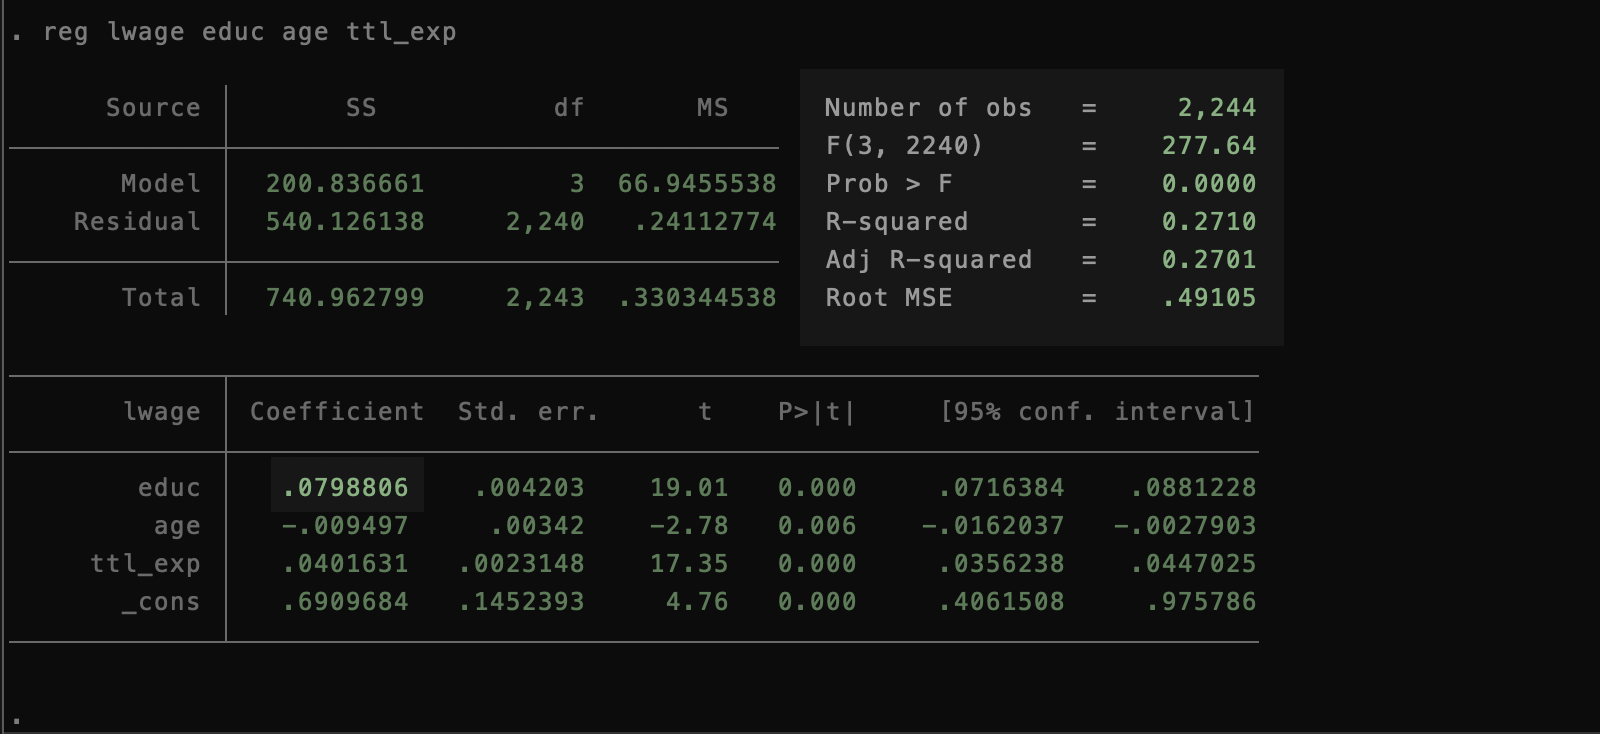
\includegraphics[width=0.4\textwidth]{inputs/reg1.png}
        \end{figure}
        \item We also get 
        \begin{itemize}
        \item The OLS estimator's standard error (square root of its variance, SE)
        \item Its $t-$statistic (ratio of coefficient and SE)
        \item Its $p-$value (Probability of obtaining an estimate at least as big as ours, and with the same sign, in a world where $\beta_1=0$ (i.e., ``under the null hypothesis''))
        \item A confidence interval where the true value of $\beta_1$ lies with 95\% probability
        \item An estimate of the intercept $\alpha$ (see the $\texttt{\_cons}$ statistic below the highlighted one)
        \end{itemize}
    \end{itemize}
\end{frame}
%---------------------------------------------------------------------

%---------------------------------------------------------------------
\begin{frame}{OLS}
    \begin{itemize}
        \item By running the simple regression command \texttt{reg lwage educ age ttl\_exp} we get:  
        \begin{figure}
            \centering
            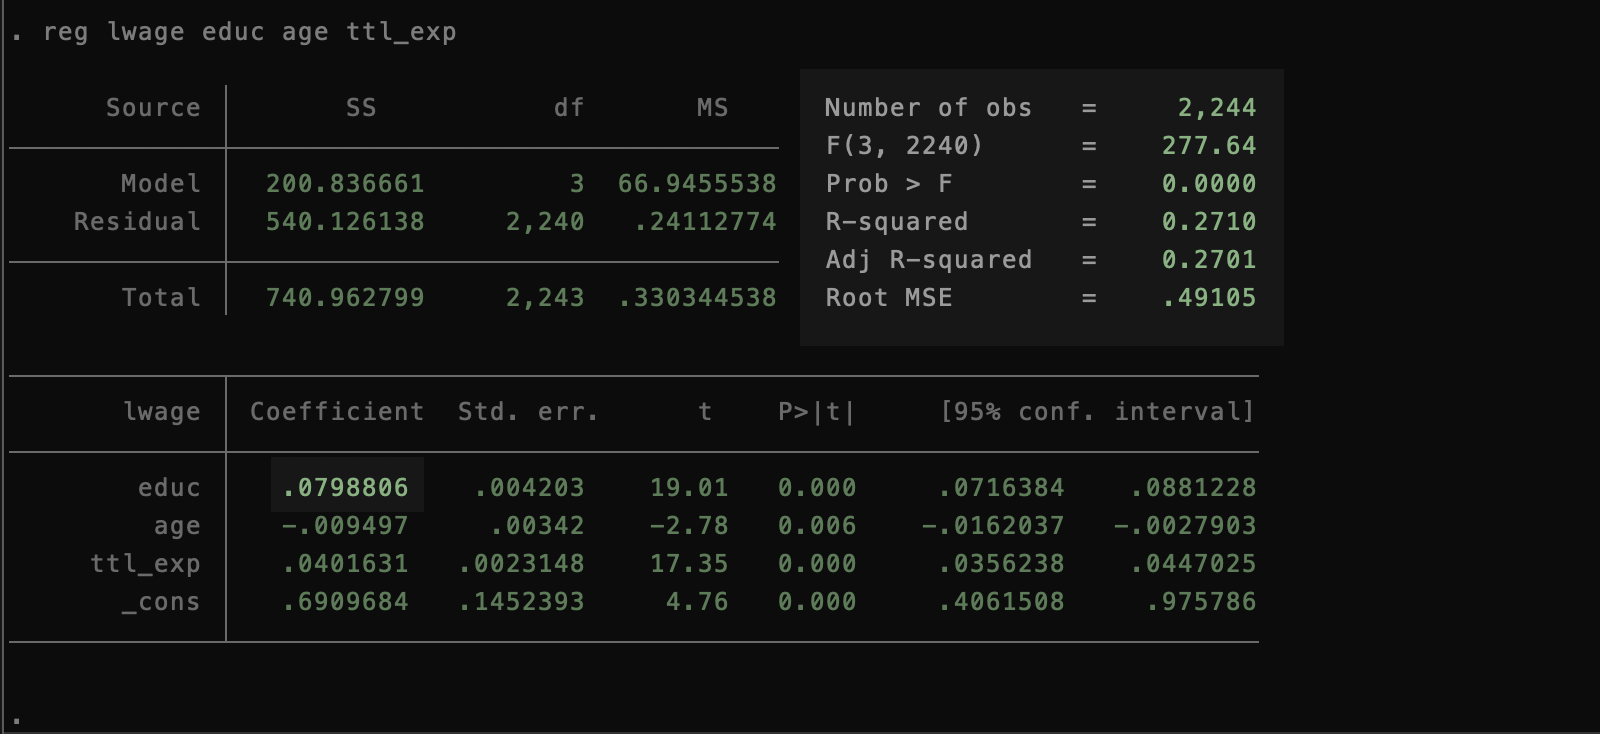
\includegraphics[width=0.4\textwidth]{inputs/reg1.png}
        \end{figure}
        \item In addition, Stata reports the regression's $R^2$
        \item This indicates the share of the variation in \texttt{lwage} that is explained by \texttt{educ}
        \item But correlation $\neq$ causation.
        \end{itemize}
\end{frame}
%---------------------------------------------------------------------

%---------------------------------------------------------------------
\begin{frame}{Binary Variables}
    \begin{itemize}
        \item Binary variables (that take only two values, for e.g., 0 or 1) are common in economics
        \item Constructing binary variables in Stata is easy:
        $$\texttt{gen collgrad = 1 if educ >= 13}$$ \\
        $$\texttt{replace collgrad = 0 if educ < 13}$$ 
        \item Or you can do it in one line:
        $$\texttt{gen collgrad = (educ >= 13)}$$
    \end{itemize}
\end{frame}
%---------------------------------------------------------------------

%---------------------------------------------------------------------
\begin{frame}{Binary Variables}
    \begin{itemize}
        \item Regressing a dependent variable on a binary variable gives us the average difference in the dependent variable between the two groups
        \item To see this, let's regress the log of wages on a binary variable indicating whether the individual is a college graduate
        \item We can do this with the command \texttt{reg lwage collgrad}
        \item Now let's also get the mean wages for college graduates and non-college graduates
    \end{itemize}
\end{frame}
%---------------------------------------------------------------------

%---------------------------------------------------------------------
% \begin{frame}{Part 4: Data Analysis -- IV}
%     \begin{itemize}
%         \item To get at the causal effects of property rights on income we need to deal with the endogeneity of institutions.
%         \item A way to do this is finding an exogenous \textbf{instrumental variable} that only affects income through its effect on institutions (details about this in lecture)
%         \item \href{https://www.aeaweb.org/articles?id=10.1257/aer.91.5.1369}{\textcolor{blue}{Acemoglu, Johnson \& Robinson (2001)}} use \textbf{log settler mortality} as their instrument 
%         \item We denote this variable by $\log M_i$, measured by \texttt{logem4} as described above.
%         \item This results in the IV model:
%                     $\log R_i = \xu + \beta \log M_i + \mathbf{X}'\delta + \nu_i \ \ \ \text{[1st Stage]}$
%             $\log y_i = \mu + \alpha R_i + \mathbf{X}'\gamma + \epsilon_i \ \ \ \ \ \ \text{[2nd Stage]}$
%         \item We can estimate $\alpha$ based on this IV model using
%             $\texttt{ivreg logpgp95 (avexpr=logem4), first}$
%         \item Stata's output will display two regression panels: one for each stage. Their structure is identical to \texttt{reg}'s output.
%         \end{itemize}
% \end{frame}
%---------------------------------------------------------------------

%---------------------------------------------------------------------
\begin{frame}
\begin{center}{\LARGE See you next time!}\end{center}
\end{frame}
%---------------------------------------------------------------------


%\beginbackup
% \appendix
%\input{sections/appendix.tex}

%\bibliographystyle{../bib/aeanobold}
%\nobibliography{../bib/bib.bib}
%\backupend


\end{document}